\documentclass[11pt, a4paper]{book}
% Warning suppression:
\usepackage{silence}
\WarningFilter*{latex}{Marginpar on page \thepage\space moved} % For comments/todo's
\WarningFilter*{caption}{Unknown document class} % Funky business with the template's caption package

% Package imports
\usepackage{svn-multi}
\svnid{$Id$}
\usepackage{prelim2e}
\renewcommand{\PrelimWords}{Draft Copy \svnkw{Id}}
\usepackage[palatino]{anuthesis}
\usepackage[hyperindex=true,
			bookmarks=true,
            pdftitle={Improving Stochastic Network Tomographic Models for Attack Detection}, 
            pdfauthor={Benjamin Sylvester Millar},
            colorlinks=false,
            pdfborder={0 0 2},
            pagebackref=false,
            citecolor=blue,
            plainpages=false,
            pdfpagelabels,
            pagebackref=true,
            hyperfootnotes=false]{hyperref}
\usepackage[all]{hypcap}
\usepackage{afterpage}
\usepackage{graphicx}
\usepackage{thesis}
\usepackage{mathtools}
\usepackage[square]{natbib}
\usepackage[normalem]{ulem}
\usepackage[table]{xcolor}
\usepackage{makeidx}
\usepackage{cleveref}
% \usepackage[style=base]{caption}
\usepackage[style=base]{subcaption}
\usepackage{float}
\usepackage{amsmath}
\usepackage{amssymb}
\usepackage[T1]{fontenc}
\usepackage[scaled]{beramono}
\usepackage{blkarray, bigstrut}
\usepackage{url}
\usepackage{multirow}
\usepackage[titletoc]{appendix}
\usepackage{tikz}
\usepackage{xparse}
\usepackage[symbols,nogroupskip,nonumberlist,sort=def]{glossaries-extra}
\usepackage{mdframed}
\usepackage{ifdraft}
\usepackage{booktabs}
\usepackage{relsize}
\usepackage{xspace}
\usepackage{listings}
\usepackage[color=todocolor, colorinlistoftodos]{todonotes}
\usepackage{setspace}
\usepackage{ifthen}


\usetikzlibrary{external}
\tikzexternalize[prefix=figs/]
\pgfkeys{/pgf/images/include external/.code=\includegraphics{#1}}

\makeatletter
\renewcommand{\todo}[2][]{\tikzexternaldisable\@todo[#1]{#2}\tikzexternalenable}
\makeatother

\urlstyle{sf}

\renewcommand{\sfdefault}{uop}
\def\UrlBreaks{\do\/\do-}

\renewcommand*{\backref}[1]{}
\renewcommand*{\backrefalt}[4]{
  \ifcase #1 %
    %
  \or
    (cited on page #2)%
  \else
    (cited on pages #2)%
  \fi
}

\crefformat{section}{\S#2#1#3}
\crefformat{subsection}{\S#2#1#3}
\crefformat{subsubsection}{\S#2#1#3}
\crefrangeformat{section}{\S\S#3#1#4 to~#5#2#6}
\crefmultiformat{section}{\S\S#2#1#3}{ and~#2#1#3}{, #2#1#3}{ and~#2#1#3}

% 
% Glossary
% 
\makenoidxglossaries
\glsxtrnewsymbol[description={The graph representing the network under analysis.}]{network}{\ensuremath{N}}
\glsxtrnewsymbol[description={Set of switches within the network $N$, analogous to link to external sub-networks}]{switches}{\ensuremath{S}}
\glsxtrnewsymbol[description={Set of monitors within the network where $M\subseteq S$}]{monitors}{\ensuremath{M}}
\glsxtrnewsymbol[description={Set of routers within the network.}]{routers}{\ensuremath{R}}
\glsxtrnewsymbol[description={Set of nefarious routers within the network $R_N\subseteq R$ that problematically hold packets.}]{nefrouters}{\ensuremath{R_N}}
\glsxtrnewsymbol[description={Cardinality of a set of network elements, or number of those within the network (i.e. |R| is the number of routers within the network).}]{|}{\ensuremath{|\;|}}
\glsxtrnewsymbol[description={The number of packets a given network element receives in a single time step}]{qlen}{\ensuremath{Q}}
\glsxtrnewsymbol[description={Set of all possible paths between monitors.}]{ppaths}{\ensuremath{P}}
\glsxtrnewsymbol[description={Set of paths between monitors which are actively probed for measurement $P^*\subseteq P$.}]{p*}{\ensuremath{P^*}} 
\glsxtrnewsymbol[description={The degree or number of links attached to a router}]{routerdeg}{\ensuremath{deg(r)}}
\glsxtrnewsymbol[description={The maximum degree of a node within a graph of subset of nodes, realised in context as $\Delta (R)$ or the maximum number of links attached to a router within the network.}]{maxdeg}{\ensuremath{\Delta}}
\glsxtrnewsymbol[description={Routers which are unidentifiable irrespective of $P^*$ under the chose routing scheme.}]{urouters}{\ensuremath{R_U}}
\glsxtrnewsymbol[description={Routers which are identifiable using some $P^*\subseteq P$ under the chose routing scheme.}]{irouters}{\ensuremath{R_I}}
\glsxtrnewsymbol[description={The maximum likelihood estimator, or the most likely set of function or model parameters $\theta$ which produced the observed outcomes.}]{mle}{\ensuremath{\hat\theta}}
\glsxtrnewsymbol[description={Set of router level metrics collected for each $r\in R_I$}]{metrics}{\ensuremath{\mathcal{M}}}
\glsxtrnewsymbol[description={The score function of a set of observations from an underlying distribution}]{score}{\ensuremath{\mathcal{S}}}
\glsxtrnewsymbol[description={The Fisher information a set of observations contains about the underlying parameters $\vec{\theta}$}]{fi}{\ensuremath{I(\vec{\theta})}}
% /glossary

%      $Id: macros.tex 506 2009-10-05 16:57:07Z daniel $   

% 
% Abbreviations
% 
\newcommand{\eg}{e.g., }
\newcommand{\ie}{i.e., }

\newcommand{\otoprule}{\midrule[\heavyrulewidth]}
\newcommand{\pdv}{Packet Delay Variation (PDV) }
\newcommand{\ur}{Uncontrollable routing (UR) }
\newcommand{\cfr}{Controllable cycle-free routing (CFR) }
\newcommand{\cbr}{Controllable cycle-based routing (CBR) }
\newcommand{\acr}{Arbitrarily controllable routing (ACR) }

\newcommand{\nurserytype}[1]{{\fontfamily{cmss}\selectfont \textsl{#1}}}
\newcommand{\alloc}{\nurserytype{allocate}\xspace}
\newcommand{\collect}{\nurserytype{collect}\xspace}
\newcommand{\redirect}{\nurserytype{redirect}\xspace}
\newcommand{\bmtype}[1]{{\textsf{#1}}}
\newcommand{\doi}[1]{\href{http://dx.doi.org/#1}{\nolinkurl{doi:#1}}}
% /Abbreviations

% 
% Math operators
% 
\DeclareMathOperator*{\argmax}{argmax}
\DeclareMathOperator*{\argmin}{argmin}
\DeclareRobustCommand{\bbone}{\text{\usefont{U}{bbold}{m}{n}1}}
\DeclareMathOperator{\EX}{\mathbb{E}}
\DeclareMathOperator{\VAR}{\hat{\mathbb{V}}}
\newcommand{\probP}{\text{I\kern-0.15em P}} 
\newtheorem{theorem}{Theorem}[section]
\newtheorem{corollary}{Corollary}[theorem]
\newtheorem{lemma}[theorem]{Lemma}
% /Math operators

% 
% Custom colours
% 
\definecolor{tableheadcolor}{rgb}{0.8,0.8,1.0}
%\definecolor{tablealtcolor}{rgb}{0.9,0.9,1.0}
\definecolor{tablealtcolor}{rgb}{0.9,0.9,0.95}
\definecolor{todocolor}{rgb}{0.8,0.8,1.0}
\definecolor{fixcolor}{rgb}{1,0.8,0.8}
\definecolor{commentcolor}{rgb}{0.8,1.0,0.8}
% /Custom colours

%
% Margin notes
%
\newcommand{\ltodo}[1]{\reversemarginpar\todo[color=todocolor]{#1}}
\newcommand{\rtodo}[1]{\normalmarginpar\todo[color=todocolor]{#1}}
\newcommand{\itodo}[1]{\todo[inline]{#1}}

\newcommand{\lfix}[1]{\reversemarginpar\todo[color=fixcolor]{#1}}
\newcommand{\rfix}[1]{\normalmarginpar\todo[color=fixcolor]{#1}}
\newcommand{\ifix}[1]{\todo[inline,color=fixcolor]{#1}}

\newcommand{\lcomment}[1]{\reversemarginpar\todo[color=commentcolor]{#1}}
\newcommand{\rcomment}[1]{\normalmarginpar\todo[color=commentcolor]{#1}}
\newcommand{\icomment}[1]{\todo[inline,color=commentcolor]{#1}}

% 
% Misc
% 

\lstloadlanguages{python}
\DeclareGraphicsRule{*}{pdf}{*}{}
\newcommand{\ignore}[1]{}
\newcommand{\mccenter}[1]{\multicolumn{1}{c|}{#1}}

\newcommand{\placeholderfigure}[2]{
\begin{figure}[ht!]
  \begin{center}
    \resizebox{\textwidth-2cm}{0.7\textwidth-1.4cm}{todo}
  \end{center}
  \caption{#2}#1
\end{figure}}

\newcommand{\rowvect}[1]{% inline row vector
  \begin{bmatrix}#1\end{bmatrix}%
}

\long\def\sfootnote[#1]#2{\begingroup%
\def\thefootnote{\fnsymbol{footnote}}\footnote[#1]{#2}\endgroup}
% /misc

%
% crossreferencing footnotes
%
%\newcommand{\fnref}[1]{~(\ref{#1})}
%\newcommand{\onecolparbox}{3.1in}


%%
%% Change the sections etc.
%%
%\makeatletter
%\parskip=0pt
%\renewcommand\section{\@startsection{section}{1}{\z@}%
%                                   {-2.5ex}% beforeskip
%%                                   {1ex}% afterskip
%                                   {\large \bfseries \raggedright}}
% \renewcommand\subsection{\@startsection{subsection}{2}{\z@}%
%                                     {-2ex\@plus -1ex \@minus -.2ex}%
%                                      {.5ex \@plus .2ex}%
%                                      {\normalsize \bfseries \raggedright}}
% \renewcommand\subsubsection{\@startsection{subsubsection}{3}{\z@}%
%                                      {-2ex\@plus -1ex \@minus -.2ex}%
%                                      {1ex \@plus .2ex}%
%                                      {\normalfont\fontsize{11pt}{12pt}\selectfont\itshape}}
%\renewcommand{\thesubsubsection}{\thesubsection.\arabic{subsubsection}}

%\renewcommand\paragraph{\@startsection{paragraph}{4}{\z@}% 
%  {.5em}%
%  {-1em}%
%  {\normalfont\normalsize\bfseries\parskip=0pt}}
%\setlength\partopsep{0\p@}
%\setlength\parskip{0\p@ \@plus \p@}

%\makeatother
%\parindent=9pt

%%% Local Variables: 
%%% mode: latex
%%% TeX-master: "doa"
%%% End:            
%%%%%%%%%%%%%%%%%%%%%%%%%%%%%%%%%%%%%%%%%%%%%%%%%%%%%%%%%%%%%%%%%%%%%%%
%% Preamble
\title{Improving Stochastic Network Tomographic Models for Attack Detection}
\author{Benjamin Sylvester Millar}
\date{\today}

\renewcommand{\thepage}{\roman{page}}

\makeindex
\begin{document}
%\doparttoc
\ActivateWarningFilters[pdftoc]
%%%%%%%%%%%%%%%%%%%%%%%%%%%%%%%%%%%%%%%%%%%%%%%%%%%%%%%%%%%%%%%%%%%%%%%
%% Title page
\pagestyle{empty}
\thispagestyle{empty}
%% anuthesis.sty Copyright (C) 1996, 1997 Steve Blackburn
%% Department of Computer Science, Australian National University
%%
\begin{titlepage}
  \enlargethispage{2cm}
  \begin{center}
    \makeatletter
    \Huge\textbf{\@title} \\[.4cm]
    \Huge\textbf{\thesisqualifier} \\[2.5cm]
    \huge\textbf{\@author} \\[9cm]
    \makeatother
    \LARGE A thesis submitted for the degree of \\
    Bachelor of Advanced Computing (Honours) \\
    The Australian National University \\[2cm]
    \thismonth
  \end{center}
\end{titlepage}


%%%%%%%%%%%%%%%%%%%%%%%%%%%%%%%%%%%%%%%%%%%%%%%%%%%%%%%%%%%%%%%%%%%%%%%
%% Todo's
\ifdraft{\listoftodos}{}

%%%%%%%%%%%%%%%%%%%%%%%%%%%%%%%%%%%%%%%%%%%%%%%%%%%%%%%%%%%%%%%%%%%%%%%
%% Here begin the preliminaries
\vspace*{14cm}
\begin{center}
  \makeatletter
  \copyright\ \@author{} 2021
  \makeatother
\end{center}
\noindent
\begin{center}
  \footnotesize{~} %\aboutthesis
\end{center}
\noindent

\newpage

\vspace*{7cm}
\begin{center}
  Except where otherwise indicated, this thesis is my own original
  work.
\end{center}

\vspace*{4cm}

\hspace{8cm}\makeatletter\@author\makeatother\par
\hspace{8cm}\today


%%%%%%%%%%%%%%%%%%%%%%%%%%%%%%%%%%%%%%%%%%%%%%%%%%%%%%%%%%%%%%%%%%%%%%%
%% Dedication
\cleardoublepage
\pagestyle{empty}
\vspace*{7cm}
\begin{center}
To my mother Kerrie, my grandparents Victor, Norma, Keith, Edna and my partner Olivia for all their support and love. 
\end{center}


%%%%%%%%%%%%%%%%%%%%%%%%%%%%%%%%%%%%%%%%%%%%%%%%%%%%%%%%%%%%%%%%%%%%%%%
%% Acknowledgements
\cleardoublepage
\pagestyle{empty}
\chapter*{Acknowledgments}
\addcontentsline{toc}{chapter}{Acknowledgments}
I acknowledge the traditional owners of the land upon which I was afforded the opportunity to complete this thesis, the Ngunnawal people. I acknowledge that this land was never ceded and and thank elders, both past and present, of the Ngunnawal people, and other first nations groups across the country.\par
Thank you to my supervisors, Ramesh and Mike, without both of your help throughout this thesis would never have gotten off the ground - much less been completed. Specifically, I want to thank Ramesh, for what has been going on three years now (wow - time flies), of guidance and advice. I also want to thank Mike, for always reminding me of the need to address the pending criticism from the person in the back of the room with their hand up - well before they have the chance to ask their question!\par
Thank you to Matthew Hole and Ashley Barnes for your assistance in helping me break though into the jargon filled world of network tomography and giving me a starting code repository, without which I would have been lost. I also want to thank Matthew for allowing me to piggy back on his Gadi project, even after receiving email warnings from NCI staff about my overly-ambitious CPU allocation requests.\par
Thank you to my gorgeous Mum, for all the phone calls checking in, always being willing to endure my whingeing about whatever had annoyed me that week, and helping me get to were I am today. Thank you to my amazing grandparents, for all your love and always believing in me. I also would be remissed if I didn't thank Garg, for taking the time to proof read this thesis, and for always being an example of organisation and perseverance to aspire to.\par
Thank you to Cole and Peter, for a great year at Scrivener street and always being around to help me switch off (sometimes perhaps a little too frequently) with an episode of Lost or some RawFM. Thank you to all my friends, from Brisbane and Canberra alike, for always being there for me (special shout-out to Ashan and El Grande Hird). And thank you to my cat Flip, for being a constant source of both comfort and irritation.\par
Last but far from least, thank you to my amazing girlfriend Olivia, for all your love and support throughout this year, all those previous, and all those to come. Without you I would have given up a long time ago. 

%%%%%%%%%%%%%%%%%%%%%%%%%%%%%%%%%%%%%%%%%%%%%%%%%%%%%%%%%%%%%%%%%%%%%%%
%% Abstract
\cleardoublepage
\pagestyle{headings}
\chapter*{Abstract}
\addcontentsline{toc}{chapter}{Abstract}
\vspace{-1em}
Network tomography is a technique used to make node-level inferences from end-to-end measurements of a network. It allows for an administrator to estimate router performance metrics without the costly overheads of traditional network monitoring approaches. We have adapted previous implementations of network tomography to estimate the queue buffer lengths of routers in stochastically routing networks, developing a technique we refer to as packet delay average (PDA) tomography. In this technique, we use the average delay of packets traversing a router as a proxy for the buffer queue length of the router. These buffer queue length estimates are subsequently used to infer the presence of \textit{nefarious routers}, which probabilistically delay packets. This probabilistic delaying represents compromised routers snooping network traffic via deep packet inspection or ex-filtrating encrypted data.\par
We have produced Python scripts for: calculation of an optimal selection of paths over the network to probe, optimal allocation of probes over these paths, and a network simulation tool using the iGraph package. We developed two classifiers (with and without access to network log files) to identify these nefarious routers in real-world ISP networks using PDA tomography. Both classifiers performed better than a random classification over all of the networks that we evaluated. An allocation of observable probe packets between paths, proportional to how many routers each was using to compute, improved classier sensitivity and specificity in two of the three networks we evaluated. Additionally, this proportional allocation increased the lower bound on the accuracy of network tomography in all tested networks.

%%%%%%%%%%%%%%%%%%%%%%%%%%%%%%%%%%%%%%%%%%%%%%%%%%%%%%%%%%%%%%%%%%%%%%%
%% Table of contents
\cleardoublepage
\pagestyle{headings}
\markboth{Contents}{Contents}
\tableofcontents
\printnoidxglossary[type=symbols,style=long,title={Notation and Terminology}]
\listoffigures
\listoftables

%%%%%%%%%%%%%%%%%%%%%%%%%%%%%%%%%%%%%%%%%%%%%%%%%%%%%%%%%%%%%%%%%%%%%%
%% Here begins the main text
\mainmatter

%% Introduction
\chapter{Introduction}
\label{cha:intro}
In this chapter, we begin by outlining the justifications behind our research into this field, highlighting the absence of current work accounting for stochastic routing in the field of network tomography in \cref{sec:Imotivationandoutline}. We then identify specific sub-problems within the existing work on stochastic routing and pose solutions to these problems
in the form of project wide scope goals.\par
Next an overview of current models and inferential techniques used in stochastic network tomography is provided in \cref{sec:Imodels}. We categorise these models into their three major components: network generation, traffic simulation, and inferential calculations.\par
In \cref{sec:Icoreconcepts} we then introduce several core concepts, each fundamental to the field of network tomography. We finally summarise topics we have introduced and key takeaways from this chapter in \cref{sec:Iintroductionsummary}.\par

\section{Outline and Motivation}
\label{sec:Imotivationandoutline}

Network tomography is the technique of using end-to-end measures to make inferences about a computer network. In this way it is similar to computed axial tomography (CAT) scans in the medical world - a process whereby x-rays are passed through a patient as a noninvasive means of gaining information pertaining to the patient's interior. These x-rays are fired from multiple points around the patient's exterior. They attenuate as they pass through different densities of tissue and are measured as they exit the body. This process results in the calculation of a single two-dimensional slice of the body's tissue density. This is typically repeated over many adjacent slices to give a 3-dimensional representation.\par
Network tomography is most analogous to a single CAT slice. However, instead of using the attenuation of x-rays to infer body tissue density, we send network packets on predefined routes between observable \textit{monitor nodes} and measure the latency of communication. This allows us to infer the structure and behaviour of routers within a network. A high level illustration of the problem is given in \ref{fig:nettom?}.\par
In network science this latency is referred to as a delay and is calculated as the time a given \textit{packet} or discrete signal takes to traverse the network to its predetermined destination. In network science there are various forms of signal casting - primarily broadcasting, uni-casting, multi-casting, and any-casting. We will focus on the case of a uni-casted signal, as the inclusion of alternative casting methods would introduce too great a complexity for one study. We note that sub-fields of research already exist for tomography under each casting method(\cite{lawrence_network_2006}).\par
\begin{figure}
    \centering
    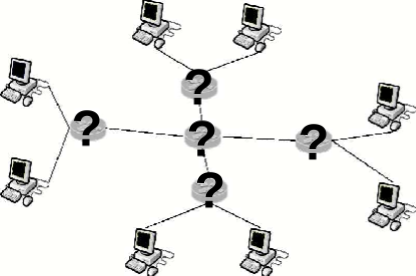
\includegraphics[width=10cm]{figs/intro/nettom-illustration.png}
    \caption[Illustrative example of network requiring tomographic probing]{Illustrative example of network requiring tomographic probing (\cite{lawrence_network_2006})}
    \label{fig:nettom?}
\end{figure}
Network tomography is primarily used for: topology identification (\cite{zhang_topology_2014}, \cite{hailiang_network_2009}), general internal state inference (\cite{vardi_network_1996}, \cite{coates_network_2001}, \cite{he_network_2021}) and, in the case of Boolean tomography, node failure localisation (\cite{nguyen_boolean_2007}, \cite{ma_optimal_2015}). In this thesis we focus on internal state inference; specifically, in the identification of abnormal behaviour of network components. Specifically, abnormal behaviour potentially caused by an attacker intent on disrupting network behaviour. This disruption of network behaviour is represented as network components problematically delaying packets they receive. This probabilistic delaying is symptomatic of a router either performing deep packet inspection on network data or ex-filtrating encrypted data which traverses the router (\cite{potteiger_evaluating_2017}, \cite{ullah_data_2018}, \cite{dorazio_data_2017}). We refer to these cases of abnormal behaviour, and the offending network components causing these, as \textit{nefarious}.\par
As network tomography advances as a discipline, it is beginning to be implemented in many real-world settings. It is now supported by emerging platforms such as Consul (\cite{shilton_network_2021}) and will see support in future network coding approaches, as discussed in \cite{kakkavas_review_2020}. The increasing use of network tomography in real-world settings therefore demands research into methods of further validating and optimising the performance of network tomography in industrial-, public- and private-communication infrastructure settings.\par
Historical work on uni-cast tomography has focused primarily on networks with an absence of queue buffers (this absence resulting in packets taking static paths through a network). \cite{lai_measuring_2000} expanded this focus by investigating routing behaviours present in stochastically routing networks. Recent work by \cite{barnes_stochastic_2020} has used the approach of \cite{lai_measuring_2000} to introduce nefarious behavior in stochastic settings and subsequently to detect such behaviours. In doing this Barnes developed a simulation more applicable to real world networks.\par
We aim to build upon this work of nefarious behaviour detection in stochastic environments. To do so, we will relax further assumptions to better simulate mid-sized complex real world networks such as a home or IoT network. We focus on ensuring that methods employed are scalable to far larger networks. In doing so, we hope to establish that the approach is generally applicable to large-scale real-world networking such as those seen in the academic, consumer ISP and commercial data center networks that underpin modern cloud infrastructure. The key assumptions upon which Barnes based their work are:\par
\begin{enumerate}
\item \emph{All packets originate and terminate at switches.}
\item \emph{All routers which are not nefarious behave identically.}
\item \emph{Packets are not dropped when traffic is heavy, instead accumulating in queues of unbound length.}
\item \emph{All end nodes are equally likely to send packets, and be chosen to receive packets.}
\item \emph{All routing protocols are the same for non-nefarious routers.}
\item \emph{Background traffic across the network has a constant average intensity.}
\item \emph{End nodes of the network are switches.}
\item \emph{The service time for every packet at the front of the queue in a router is 1 “time step”.}
\end{enumerate}

We focus on the relaxation of assumptions 1-5, and leave future work to address additional assumptions. Each of these assumptions is relaxed within our python based network simulation tool. The programmatic functionality which enables their relaxation is covered in \cref{cha:methodology}.\par
We choose not to relax assumption 6 as it allows for a bounded network size. Without switches as end nodes we would be forced to instead recursively model all connected sub-networks. This would eventually lead to a model that represented the entire observable internet connected to this network; being unbounded in size, this would be both impractical and of little use to analyse.\par
We choose not to relax assumption 7 as it allows for analysis of arbitrary sub-networks that may be of interest to the typical network administrator. Adjacent networks can be represented as single node with a number of switches connected proportional to the typical traffic from that network.\par
We chose not to relax assumption 8, as it is key to the analysis technique used within our work. The difficulty behind its relaxation is expanded in \cref{sec:Rnefarouterdetection}, and the relaxation of this particular assumption is left to further work on the topic.\par
In relaxing these assumptions and implementing extensions, we hypothesise that network tomography can be used to estimate routers' buffer queue lengths with sufficient accuracy to enable inference of packet delaying behaviour by individual routers within real world networks. Due to the large scope of this hypothesis, we decompose it into 2 sub-hypothesis:
\begin{enumerate}
    \item Network tomography enables inference of node level packet delay metrics within stochastically routing real-world networks.
    \item A router can be classified as exhibiting nefarious behaviour or not by using information gained from packet delay metrics.
\end{enumerate}
As real-world use of network tomography is exponentially more complex than previous mathematical models (\cite{barnes_stochastic_2020}), in tackling sub-hypothesis 1 we introduce an alternative and novel method of packet delay average (PDA) tomography (\cref{sssec:Iinferentialcalculations}). To evaluate sub-hypothesis 2, we perform a series of experiments that vary network parameters (\cref{sec:MNefidentification}). From these we develop three binary classifiers to identify nefarious routers under three sets of assumptions. We evaluate each of these classifiers against the requirements of three real-world use cases.\par
Compared to previous theoretical methods, our approach classifies nefarious nodes less accurately and less precisely. However, we utilise optimization techniques (presented in \cref{sec:Boptimization}) to maximise the accuracy of our novel methods. To measure the impact of optimisations, we quantify the maximum potential accuracy of our inferences using statistical methods from link-focused tomography, as outlined in \cite{he_fisher_2015}. We represent all known information about the network using its Fisher information (see \cref{ssec:Bfisherinformation}). This representation results in the maximum potential accuracy of our analysis being given by the Cramér–Rao Bound (see \cref{ssec:Bcrb}).\par
Additionally we hope this work on the power of tomography in an adversarial setting will spur interest in the fledgling field of adversarial tomography. We note that few studies on the topic have been conducted to date (\cite{he_network_2021}) and believe further research in this area could be extremely beneficial to the security and networking communities.

\section{Stochastic Network Tomographic Models}
\label{sec:Imodels}

In this section, we introduce existing models and methods for stochastic network tomography in literature. For ease of discussion, we split these models into three sections: network generation, traffic simulation and inferential calculations. This decomposition was chosen as each section can be treated as a distinct process, with the output from each able to be parsed to the next in a context-free manner. In \cref{ssec:Icurrentmodels} we cover specific methods currently used for each of these three areas. Additionally, in this section, we address traffic and delay simulation, highlighting assumptions and key segments for potential improvement in current models. Finally we provide an overview of the model produced as a key deliverable of this project, outlining differences from the current work.

\subsection{Previous Models}
\label{ssec:Icurrentmodels}

Previous work surrounding network tomographic models identifying nefarious nodes in stochastic networks is led by \cite{barnes_stochastic_2020}. This work takes a theoretical mathematical approach to tomography, and was based upon the requirement that the system be described by a formal mathematical model. In this section we introduce approaches used in Barnes's work along with candidate areas considered for extension. We provide additional explanation and background of these techniques in \cref{cha:background}. We note that work in both \cite{he_fisher_2015} and \cite{kolar_distributed_2020} also covers stochastic environments. Both these studies, however, focus on link level metrics. Notwithstanding this, in  \cref{ssec:Idevelopedmodels} we show how techniques from previous work on link metrics can be adapted for use in our setting.

\subsubsection*{Network Generation}
\label{sssec:Inetworkgeneration}

The goal of network generation in the context of validating tomographic models is the production of a random undirected graph representing a small to medium sized network. The generated network must contain four essential components: 
\begin{enumerate}
    \item \textit{Routers} to direct packets.
    \item \textit{Switches} to emulate connection to a larger external network (i.e. the world wide web) or end points, through stochastic production of packets (elaborated upon in \cref{sssec:Itrafficsimulation}), and reception packets.
    \item \textit{Monitors} which are particular switches we are able to directly control and observe.
    \item \textit{Links} between routers for packets to traverse.
\end{enumerate}
Components 1, 2, and 3 are represented as nodes within the graph, and component 4 is represented by edges between nodes. The generation of these pseudo-random networks is desirable for verification of tomographic techniques in a controlled environment as it allows for many topologies to be tested, thereby ensuring the robustness of introduced techniques.\par
Previous work around nefarious router identification in stochastic networks (by \cite{barnes_stochastic_2020}) employs a user-defined connectivity parameter to generate edges between nodes. This is analogous to the Erdos-Renyi (ER) generation technique originally posed in \cite{erdos_random_1959}. We provide formal definitions of this technique in \cref{sec:Bgraphgeneration}. In real-world networks, however, router degree (the number of connected routers and switches) converges to a power law (\cite{chen_origin_2002}, \cite{zhao_measurement_2020}). Such graphs are commonly referred to as scale-free. In contrast to this, a Poisson distribution of node degree is observed in other, more naive, network generation algorithms such as the Erdős–Rényi model. A comparison of node degree between graphs generated with an ER technique and those generated with a scale free technique is given in \cref{fig:nddist} where, $P(k)$ is the probability of a in a network node having degree ($k$).\par
\begin{figure}[t]
    \centering
    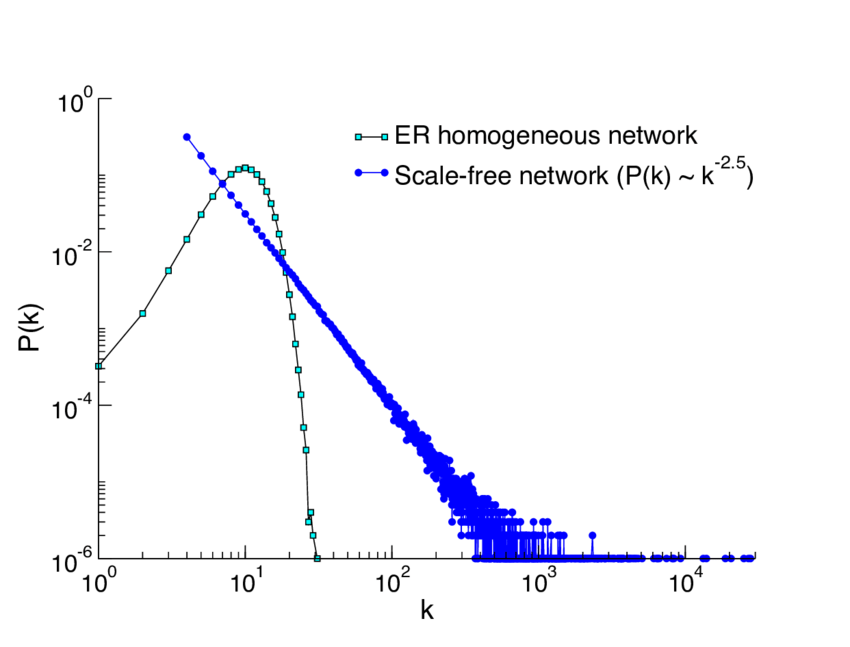
\includegraphics[width=10cm]{figs/intro/nodedegree-dist.png}
    \caption[Distribution of node degree in a generated network]{Distribution of node degree in a generated network \cite{baronchelli_networks_2013}}
    \label{fig:nddist}
\end{figure}
Existing work on stochastic network tomography - primarily from \cite{thoppe_stochastic_2014} \cite{kolar_distributed_2020} - represents networks in a tree-based topology. As noted in \cref{cha:litreview}, the adoption of this technique is common practice when utilizing multi-cast packet transmission for inferential calculations. Such tree-based models, although useful for simplifying tomographic problems, are poor representations of real systems.

\subsubsection*{Traffic Simulation}
\label{sssec:Itrafficsimulation}

The accumulation of all packets sent between each node in the network (referred to as \textit{network traffic} or simply \textit{traffic}) and its simulation is a key aspect of any network model. The traffic within a network is an accumulation of all packets sent from each switch within that network. The traffic at any single router is therefore determined by the number of components adjacent to it, their respective routing tables, and the number of packets forwarded to them. The current model used within the work of \cite{barnes_stochastic_2020} splits traffic simulation into discrete time steps of a uniform length. We adopt their assumption that each time step is a period small enough that only a single packet is handled by each router in each step.\par
Due to this discretization of network traffic, packets (as one would anticipate) do not traverse instantly from sender to receiver, but rather are delayed at various points along their path. We adopt terminology from the authoritative work of \cite{kurose_computer_2013}, and decompose this delay into four classes:
\begin{itemize}
    \item Processing delay
    \item Transmission delay
    \item Propagation delay
    \item Queuing delay
\end{itemize}
Processing delay is the time required for a network component to analyse the requirements of a packet and then take action on those requirements. Transmission delay is the time taken for the link interface of a network component to transmit the physical bits representing the information onto the transmission interface (i.e. fibre, copper, wireless). Propagation delay is the time taken for the signal to traverse the transmission interface from sender to receiver. This is largely dependent on the type of medium and the physical distance between components. Lastly, queuing delay, for the purposes of our work is defined as the delay a packet experiences while waiting in the buffer of a router.\par
In existing models multiple packets may be forwarded to a single router each time step, and each router is only able to perform one forward per time step. Therefore these packets can accumulate in the respective routers’ queues, awaiting forwarding. These router queue lengths are analogous to queuing-delays in real world systems. The work of \cite{barnes_stochastic_2020} considers only the class of queuing delays when dealing with packet delay measurements, where other work on stochastic tomography (\cite{kolar_distributed_2020}, \cite{he_fisher_2015}) makes no distinction between delay classes, instead dealing only with the generalised concept. As noted in \cite{telchemy_impact_2006}, propagation and processing delays are negligible in realistic applications. We therefore focus primarily on extending the work of \cite{barnes_stochastic_2020} and their focus on queuing delays.\par
Although all packets in a network experience queuing delays, the magnitude of the delay is ultimately dependent on the number of packets within the system at any given point in time; or as it is commonly referred to, the network's \textit{traffic intensity}. Traffic intensity is a result of the number of packets sent over a network by switches.\par
The number of packets a switch sends each time step has been shown to have a binomial distribution (\cite{barnes_stochastic_2020}) over a set time window. This approaches a Poisson distribution over a large enough number of time steps. From (\cite{barnes_stochastic_2020}), where $n$ denotes the number of time steps, $k$ being the number of packets sent and $s$ being the probability on any given time step that a packet will be sent:
\[\lim_{n\to\infty} \frac{n!}{k!(n-k)!}s^k (1-s)^{n-k} =\frac{s^k e^{-s}}{k!}\]
This known distribution of traffic intensity is key in existing work as it allows for the traffic being sent from a node to be represented as a random variable S with a known distribution and a value of one or zero, depending on whether a packet is sent or not.\par
Prior work assuming constant average traffic intensity has shown that queue lengths, and, consequently, queuing delay converge to a steady state over time. Additionally, given a queue length's dependency on the queue length at the previous time step, it has been shown to be a Markov process (\cite{barnes_stochastic_2020}). However, the queue length for each router is a consequence not only of the number of packets sent, but also of the paths these packets take through the network. Therefore, the routing method used by the network must be scrutinised so as to utilize a Markov chain model and thus represent queuing delay as a random variable, as shown in \cite{barnes_stochastic_2020}.\par
For network traffic to be stochastic, any routing protocol must be dynamic in nature. If routing tables were fixed, only a single constant path would be taken by a packet between any two nodes. This would result in traffic variations being solely a product of the packet generation rate of switches. Previous work uses an abstract implementation of the distance-vector routing protocol (\cite{perkins_ad_2003}) to achieve this dynamic routing behaviour. This was accomplished using a global controller to compute the shortest distance between any two nodes using Dijkstra's algorithm and broadcasts this information to all components in the network (\cite{barnes_stochastic_2020}). In Barnes's method the weight of an edge represents the number of packets in the queue of the connected router. This representation is valid, as the queue length is analogous to the number of time steps a packet would wait before completing its traversal of that edge.\par
The use of a network-wide controller in this manner is akin to that of Software Defined Networks (SDNs) where routing logic at the link level is dynamically handled by an SDN controller (see \cite{kreutz_software-defined_2015}). Due to most commercial-grade networks not currently employing SDNs and, to the myriad of security concerns surrounding widespread adoption of SDN technology (\cite{wood_scalable_2021}), we highlight the decentralization of this background traffic routing as a key area of work addressed in \cref{sec:Broutingmechanisms}.\par
Additionally, in the work of \cite{barnes_stochastic_2020}, no distinction is made at a routing level between different types of traffic that the router is forwarding. A packet sent by a monitor node, that we are able to draw inference from, is treated identically to all other packets. As in \cref{sec:Mnetworkprobing}, we adopt the terminology of \cite{he_network_2021} and refer to this as uncontrolled routing (UR). UR is characterised by observable packets sent between monitor nodes following the underlying routing behaviour of the network. However, modern routers are able to make distinctions between different types of packets and so forward them accordingly. Therefore alternate routing of probe packets is feasible under both normal and SDN conditions. Due to our model varying only the routing restriction for probe packets, we use the term \textit{routing} to refer exclusively to the routing of probe packets. We refer to all non-probe traffic as \textit{background traffic}. We introduce alternative forms of routing (originally presented in \cite{he_network_2021}) in \cref{sec:Broutingmechanisms}, as key targets for extension of the existing model.

\subsubsection*{Inferential Calculations}
\label{sssec:Iinferentialcalculations}

In previous models packets are collected at each monitor node throughout the simulation. The cumulative packet delay distribution for each monitor is then computed at the end of the simulation. This calculation of packet delays is trivial. As packets traverse between monitors both the time they are sent from and the time they arrive at monitors is known. However, the path each packet takes through the network is unknown and uncontrollable (due to UR). Due to this, the only method of identifying nefarious routers is to compute expected delay distributions resulting from every possible subset nefarious of routers and compare these to the observed delay distributions.\par
However, the computation of an expected delay distribution is non-trivial as it is dependent on $q$, the number of simulated time steps, and the topology of the network. As presented in \cref{ssec:Icurrentmodels}, one solution (from \cite{barnes_stochastic_2020}), utilises a combined agent-based and Markov Chain Monte Carlo (MCMC) approach for calculating these expected delay distributions.\par
The resulting delay distribution is then compared to the observed delay distribution using techniques from signal analysis (presented in \cite{lynn_introduction_2016}). A correlation metric $C$ is computed, where $C(D_x,D_y)=0$ if $D_x$ has an identical distribution to $D_y$. In this comparison both distributions are probability density functions (PDFs) normalised via L2 normalization to yield the Euclidean norm. This method allows for extremely accurate calculation of nefarious nodes compared to conventional methods of link inference tomography.\par
As this correlation is the sole usable method to gain inference, this approach is extremely domain dependant, unable to detect nefarious behaviour if deployed in a network with a single node different from where it was constructed. Additionally, it is prohibitively expensive to infer packet delay metrics by calculating all candidate PDFs for every possible configuration of nefarious routers.\par
The computation of expected delay distributions for each subset of nefarious routers takes on the order of number of router combinations $\mathcal{O}(2^{|R|})$. Previous work in \cite{belloni_computational_2009} has established the complexity of an MCMC algorithm over a large sample space as $\mathcal{O}(d^3 log d)$ where d is the dimensionality of the sample space, or network in our case, which is known to be $\leq 2\cdot \Delta N + 1$ (\cite{erdos_chromatic_1980}). The total complexity of this method is therefore on the order of:
\begin{align}
\label{eq:mcmcbigo}
    \begin{split}
        &\mathcal{O}( (2\cdot \Delta N + 1)^3 \cdot log(2\cdot \Delta N + 1)\cdot 2^{|R|})\\
        &\mathcal{O}(\Delta N ^3 \cdot log \Delta N \cdot 2^{|R|})
    \end{split}
\end{align}\par
However, one drawback noted in the development of this solution was its sensitivity to network hyperparameters, such as traffic flow and queue length. An alternative approach (in \cite{kolar_distributed_2020}) utilizes a distributed scheme to achieve an inferential time complexity of $\mathcal{O}((NPR)^3)$. Data transfer costs and duplicate computations between nodes in this scheme, however, result in the real-world performance being far worse than this theoretical complexity would indicate (\cite{kolar_distributed_2020}).\par
We therefore aim to establish the use of routing techniques other than UR along with new inference techniques of PD tomography to optimize identification of nefarious routers.\par

\subsection{Developed Model}
\label{ssec:Idevelopedmodels}
As a part of this work, we have developed a network tomographic model using python for bespoke simulation in a constrained environment. The main adaptations over the precious model, covered in \cref{sec:Broutingmechanisms}, are: decentralization of background routing logic, and distinction of probe packets from background traffic. Additionally we implement two optimisations in the model: selection of a minimal set of paths over which to send probe packets, and probabilistic injection of probe packets over each of these paths. We elaborate on these in \cref{sec:Boptimization}.\par
These additions were made to enable packet delay average (PDA) tomography (outlined in \cref{sec:Mnetworkprobing}) to be used in inferential analysis. Finally we highlight minor features, attention to which might better emulate real-world network behaviour. One such feature is the halting of probe injection before the end of the simulation run-time (\cref{sec:Mnetworkprobing}). This halting is intended to represent real-world situations where an administrator would run a network diagnostic for a set amount of time while the network is under load. We refer to this period of actively probing the network as a \textit{measurement interval}.

\section{Core Concepts}
\label{sec:Icoreconcepts}

In this section we describe how network tomography is able to be posed as an inverse problem, and why this is useful. We introduce generalised concepts of stochastic parameter estimation using inverse approaches, namely, Fisher information and optimization techniques. We give a lower-level explanation of how the Fisher information is computed in \cref{cha:background}. Finally we show how these techniques and their results can be applied directly within the context of our work in (\cref{cha:methodology}) to evaluate the efficacy of our approach.\par
At the most basic level, an inverse problem is one where observations must be used to determine unknown causal factors (\cref{fig:probleminv}, \cite{sadri_effect_2019}). In the context of tomography, packet-level information is observed at monitors and underlying network parameters are calculated; or rather, in the case of stochastic tomography, estimated. Application of network tomography in this manner enables system administrators to monitor for nefarious routers with less traffic overhead and with less system modification, as compared to more conventional methods.\par
\begin{figure}
    \centering
    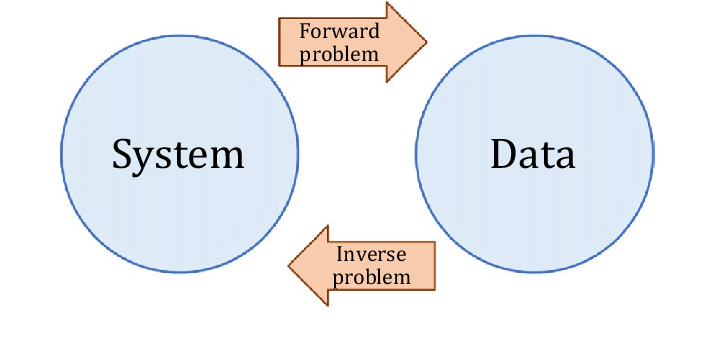
\includegraphics[width=10cm]{figs/intro/inverse_problems.png}
    \caption[Illustration of problem inversion]{Illustration of problem inversion \cite{sadri_effect_2019}}
    \label{fig:probleminv}
\end{figure}
As noted in \cref{sec:Imotivationandoutline}, we aim specifically to infer, via observation of packet delay, the presence and location of nefariously delaying routers within a network. We expect the distribution of packet delays, for nefarious nodes, to be more varied and have a heavier tail due to the delaying of packets.\par
To optimize stochastic network tomography, we must consider how to maximise the accuracy of our analysis given the random nature of the network. Intuitively the accuracy of our analysis is limited by the amount of information we are able to collate from our probing. We employ the concept of Fisher information (see \cref{ssec:Bfisherinformation}) from the field of statistical signal detection (\cite{poor_introduction_1994}) to represent our knowledge of a single element of the network.\par
It follows that the garnered information of all elements in the network can be presented in a Fisher information matrix (FIM) to concretely represent our knowledge of all network elements. As we are primarily measuring the average delay of packets within the network, the FIM represents the information we have about queuing delays of individual routers. This is intrinsically related to the paths we have designated probes to take through that network.\par
In addition to quantifying our knowledge of a network, the FIM has the secondary property of being able to quantify the minimum accuracy of estimations made about the system it represents. This lower bound on the accuracy of inferential estimations is known as the Cramér–Rao bound (CRB). The CRB represents the worst possible inference we can make about a router's queuing delays given collected probing measurements. In \cref{sec:Bparameterestimation} we provide formal definitions of FIM's and their corresponding CRB. We extend on these formal definitions in \cref{sec:Boptimization} to show how the CRB can be improved through optimisations to probe path selection. We additionally consider optimisations to the allocation of probes between these paths. To accomplish this, techniques of optimal experiment design (\cite{anthony_c_optimum_1996}) are introduced (in \cref{sec:Boptimization}) and then used (in \cref{sec:Mnetworkprobing}) to maximise inferential accuracy via probe allocation over paths.\par

\section{Summary}
\label{sec:Iintroductionsummary}

In this section we have posed the problem of improving existing network tomography simulations. We noted the utility of approaching this goal as three separate but related problems of: metric inference, information processing, and optimisation. We formally posed an overarching hypothesis that network tomography can be used to estimate routers' buffer queue lengths with sufficient accuracy as to enable inference of packet delaying behaviour by individual routers within real world networks. To better fit our decomposition of the problem, we broke this hypothesis into two independent sub-hypotheses.\par
We introduced previous models of network tomography in stochastic networks, decomposing these models into three sections: network generation, traffic simulation, and inferential calculation. We highlighted the lack of applicability to general topologies and computational intensity of these models as our focus for improvement. 
Optimisation to the code for computational were noted as desirable, as they enable extended simulation run time allowing statistical approximations to converge. The ability to handle general topologies is a key requirement for addressing our hypothesis as it allows for simulation and fair comparison of real world national ISP networks. The final artefact of code is made available at (\cite{sylvester_millar_real_2021}) in hopes that future work will then be able to further expand on this area of work. Specific candidates for future extensions are highlighted in \cref{cha:conc}.

%% Chapters
\chapter{Literature Review}
\label{cha:litreview}

The term network tomography first came into use in \cite{vardi_network_1996}, focusing on the estimation of network traffic intensity from individual link data. This estimation is accomplished using a known routing table and frequent measurements of link traffic under an assumed (Poisson) distribution. These techniques are lifted directly from related work examining statistical properties of Positron Emission Tomography in the medical field (Used in PET scans) (\cite{vardi_statistical_1985}). This allows for the internal state of a network to be reconstructed using only peripheral measurements and as such is extremely useful in cases of network monitoring where no access to internal nodes is required; eg. in subsections of the internet or large GPONs such as the National Broadband Network (NBN) (\cite{gregory_how_2019}).\par
Early work in the field (such as Vardi’s) also touches on the notion of deterministic or Markovian routing. Specifically, under the assumption that fixed routing can be considered a special case of deterministic routing and, as such, that both can be solved given the same set of predefined assumptions. The problem of tomography was originally presented as a ‘LININPOS’ or LINear INverse POSitive problem, and only explored as a purely statistical matter. Using a more practical lens, we would now term this as a form of passive tomography.\par
Shortly after this initial statistical paper, the study of the emerging field of network tomography (referred to hereafter simply as tomography) split into two related but distinct approaches; that of statisticians/mathematicians, and that of computer scientists.\par
Computer scientists further decomposed tomography into passive and active tomography. Passive tomography uses measurements aggregated from observations of all network traffic so as to calculate properties such as traffic intensity (\cite{vardi_network_1996}, \cite{coates_network_2001}) and network topology (\cite{hailiang_network_2009}, \cite{zhang_topology_2014}, \cite{hailiang_network_2009}).\par
The determination of source-destination traffic intensity is often referred to as traffic matrix or origin destination tomography. This branch of network tomography focuses on aggregation of internal link measurements to determine network wide traffic intensity (\cite{cao_time-varying_2000}). In contrast, network topology identification focuses on forming a best-effort approximation of all node-to-node connections based on observed distance metrics.\par
As each of these approaches require access to all network traffic, they require a set of edge routers from which this traffic can be observed. However, such a set is not always obtainable in real-world situations due to hurdles such as traffic anonymization (preventing capture of packet sources) and the large proportion of edge routers required to be controlled by an observer (limiting scalability) (\cite{leung_measurement-based_2002}). In contrast, active tomography is more applicable to real-world systems as it requires less assumed knowledge of the network's state and also less access to components of the network.\par
Active tomography, commonly referred to within literature as either Quality of Service (QoS) tomography or network performance tomography (\cite{lawrence_network_2006}, \cite{barnes_stochastic_2020}), can be subdivided into two main approaches of boolean and additive tomography. Each of these approaches is characterised by its representation of internal performance. Additionally, each approach results in different performance metrics being exposed for evaluation.\par
Boolean tomography represents the internal state of links as an unknown boolean variable. In the conventional case of failure localisation, this variable corresponds to a “normal” and “failed” state. Therefore, the inverse problem arises from the success/failure of a source destination path being the logical OR of its composite paths (\cite{duffield_network_2006}). In contrast, additive tomography represents the internal state of links as an unknown non-negative value so as to model non-binary performance metrics (primarily link delay). Given this representation in additive tomography, the inverse problem arises from the total delay on a path being the sum of all delays of its composite paths. Although boolean and additive tomography have many differences in goals and methodologies, there are some similarities between them. Specifically, in the conditions sufficient to allow for inferences to be drawn. \par
The topological conditions under which inferences are able to be made in both additive and boolean tomography vary depending on which routing policy is used for monitor probes. A derivation of these conditions is given in \cite{he_network_2021}. We summarise and present these conditions under different routing mechanisms in \cref{sec:Broutingmechanisms}. Regardless of routing conditions, in both additive and link tomography, end-to-end measures are used to infer individual link level performance characteristics of the network. All work up to this point has focused on the notion of deterministic link performance. However, in real world networks this assumption is seldom correct.\par
The investigation of stochastic performance on router links, and consequently on routing behaviours, has become increasingly popular in recent years. The use of tomography to draw link level performance inferences in such an environment is termed stochastic network tomography. Most current work on the topic, like that of active tomography, can be split into the two subcategories of boolean and non-boolean. Both these techniques seek to identify the distribution of associated metrics according to an unknown parameter $\theta$. The goal of tomography is therefore to estimate $\theta$ from end-to-end observations (\cite{he_fisher_2015}).\par
Boolean stochastic tomography focuses on the packet loss of a network where packets are non-deterministically dropped from the network (potentially due to an intermittent node or link failure). In contrast, non-boolean stochastic tomography looks to infer information around expected delays on each link (possibly caused by signal congestion or signal handling techniques such as deep packet inspection (\cite{el-maghraby_survey_2017})). Both these tasks are accomplished by using Fisher information matrices (FIM) with known and controllable routes to develop Maximum Likelihood Estimators (MLEs). The specifics of this technique are covered in detail in \cref{sec:Bparameterestimation}.\par
Alongside development of new network tomography techniques, research has been undertaken to optimise existing applications of network tomography. The most notable work surrounding optimisation has been around the selection of which set paths between monitors to probe. This work is notable as optimisation to selection of probe paths can reduce the traffic overhead required to generate accurate results using network tomography. This problem has been approached from three distinct directions in the works of \cite{zheng_minimizing_2013}, \cite{tootaghaj_parsimonious_2018}, and \cite{rahali_unicast_2019}.\par
In their 2013 study of link performance monitoring techniques, \cite{zheng_minimizing_2013}, developed an algorithm to select a minimal set of path between monitors which still allow routers to be identified using network tomography. In contrast, the Greedy-Min-Cost-Rank (GMCR) algorithm was developed in \cite{tootaghaj_parsimonious_2018} to select a set of paths between monitors with the smallest possible number of links across all paths. Most recently, the k-paths method (an extension of the work of \cite{lawrence_network_2006}) and the Evolutionary Sampling algorithm (ESA) were developed in \cite{rahali_unicast_2019}, with the goal of selecting the minimal set of paths between monitors.\par
We note that ESA, developed as an extension to k-paths, dominated k-paths in both computational efficiency and accuracy. This was due to their use of a technique based on random sampling designed to avoid the high computation and memory complexity. Additionally, both of these solutions accounted for the costs associated with the collation of metrics from all monitors at a single location post-analysis.\par
Finally, in the work of \cite{barnes_stochastic_2020} the use of tomography to infer link level performance in a stochastic system was foregone in favour of the ability to identify nefarious nodes. This was accomplished through the development of a mathematical model to simulate expected queue lengths at nodes, given all possible configurations of nefarious routers. Nefarious routers in this work are represented as having a probability, at any discrete time step, of not forwarding a packet to another router. The delay distributions generated by the MCMC model are then compared to that observed at monitor nodes. The most closely correlated is shown to be a correct prediction of the set of nefarious routers. The primary goal of our work is to apply techniques of packet delay estimation so as to improve the efficacy and efficiency of this nefarious router identification.\par
\chapter{Background}
\label{cha:background}

In this chapter we aim to provide the reader with a concrete understanding of key concepts within our new tomographic technique. Descriptions of metrics and methods used to analyse and verify the technique are also introduced. We begin with the theory and intuition behind previously used random network generation algorithms in \cref{sec:Bgraphgeneration}.\par
We establish the requirement for discriminatory probe path routing within the network and draw real world analogues for hypothetical routing constraints in \cref{sec:Broutingmechanisms}. Routing is separated into four classes according to these restraints and a focus on the \cbr and \cfr mechanisms for subsequent sections is established.\par
We then cover key statistical concepts, summarising their realisation within our work in \cref{sec:Bparameterestimation} and \cref{sec:Boptimization}. Lastly we tie all aforementioned concepts together through their use within our novel tomographic model and explore previous implementations of \pdv tomography within the network tomographic corpus in \cref{sec:Mnetworkprobing}.

\section{Graph Generation}
\label{sec:Bgraphgeneration}

Monitors in the case of this model function as normal switches with regards to packet generation and reception but perform additional recording functionality. Each monitor stores information pertaining to each packet which is generated or received by itself. This stored information is analogous to a traceroute of the packet's path through the network; a list of routers that the packet has passed through. The monitors also store the total time taken by the packet for it’s traversal, as well as the source and destination IP.\par
Within the graph resulting from the network generation, all edges are undirected and represent links between machines (router, switches or monitors). For simplicity each distinct pair of nodes may only be linked by a single edge, however multiple physical links between a pair of machines occur in the real world, the edge can be considered a virtual aggregation of all of these links, representing their total cumulative throughput. Each node within the graph is a representation of a physical piece of networking hardware, either a router or switch, these are simplified abstractions of their real world analogous, with their key simplifications being those enumerated in the previous section.\par
The current network generation strategy follows that of the Erdős–Rényi (ER) model; this was introduced by \cite{gilbert_random_1961} and later that year revisited in “On Random Graphs I.” by the model’s titular author pair \cite{erdos_random_1959}. This random graph generation is characterised by each node in a graph being connected to each other node with a predefined probability of $p$, that is for a graph \gls{network} with $n>1$ nodes and a connectivity probability $0\leq p\leq 1$, $G=f(n,p)$.\par
This random graph generation strategy is intuitive in its simplicity however has several problems when used to generate graphs analogous to computer networks. The most prominent shortcomings are in the node degree distribution and presence of so called ‘isolated nodes’. A key underlying assumption of the ER model is that each edge between two nodes is equally likely to occur within a graph. The natural consequence of this assumption is that the distribution of node degree’s (number of connected edges) within the graph approximates a Poisson distribution (\cite{albert-laszlo_scale-free_2003}). Such random networks are referred to as exponential networks as the probability that a node is connected to $n$ other nodes decreases exponentially as $n\to\infty$.\par
Complex networks however have not been observed to follow a random pattern but rather that, irrelevant of age, function or scope converge to a similar architecture as shown in \cite{albert_diameter_1999}’s mapping of the world wide web . This network architecture has been dubbed as scale-free and is characterised by the distribution of node degree following a power-law where the probability of a node having $k$ edges $P(k)$  is proportional to $\frac{1}{kn}$ for a network of $n$ nodes. This property is present in graphs generated using the Barabási–Albert (BA) model, as well as the Watts–Strogatz model; these generation techniques among others are further discussed in \cref{cha:background}.\par
As the network being generated and analyzed continues to increase in size we expect its behaviour and structure to become increasingly complex. Given this complex nature the scale-free property of graph generation is highly desirable for generation of pseudo realistic networks.

\section{Routing Mechanisms}
\label{sec:Broutingmechanisms}

    In this work we use the term probe packets to denote UDP packets sent between monitors which differ from other traffic by their transfer from and to uniquely identifiable ports on the sending and receiving switch. Probe packets are allocated on a per packet basis to a unique path through the network (referred to as a probe path) which is a directed path through a series of routers which the packet is guaranteed to take by the routing protocols unless it is dropped due to a router buffer within the path being full. Each probe path in the set of selected probe paths (denoted as $P$) is uniquely identified by the monitors it is between and the set of routers it traverses. The probe path a packet is taking is noted though the packet's respective transmission/reception port and additional explicit notation within the data section of the packet, we further elaborate on the technical representation of these probe paths in \cref{sec:Mnetworkprobing}.\par
    
    Given we assume a priori knowledge of the network's topology a set of probe paths is decided on before beginning to collect end-to-end measurements. At the beginning of the measurement interval each monitor sends an allocated number of probe packets along each probe path, noting the time sent ($t^s$) and along which probe path. The destination monitor upon reception of the packet then also stores the time of reception ($t^r$) and packet's probe path, as illustrated in \ref{fig:pptransmission}. 
    \begin{figure}[H]
        \centering
        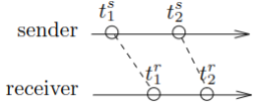
\includegraphics[width=5cm]{figs/background/probe_transmission.png}
        \caption[Illustration of probe packet transmission between two monitors]{Illustration of probe packet transmission between two monitors \protect\cite{he_fisher_2015}}
        \label{fig:pptransmission}
    \end{figure}
    \noindent Given $n$ probes are sent on a path we are then able to find the mean end-to-end travel time of a packet on that path by: \[\text{travel time}=\frac{\sum_{i=1}^nt_i^r - t_i^s}{n}\] where $t_n^s$, $t_n^r$ denote the time the $x$th packet sent on that path is sent and received respectively. This calculation is trivial within small networks as there exist only a small number of probe paths and the measurement interval (and therefore $n$) required for reliable metrics is brief. To account for clock synchronization discrepancies between distributed monitors in this calculation we introduce the concept of packet delay variation (PDV) tomography for analysis in \cref{sec:Mnetworkprobing} \par

    Let \gls{monitors} denote the set of monitors within \gls{network}, \gls{ppaths} denote the set of all possible probe paths, and $\gls{|}P|$ be the number of potential probe paths  is then intuitively equal to all possible non cyclic paths between each pair of monitors. A naive approach of calculating all probe paths is therefore of the order $\mathcal{O}(m^m)$ where $m=\gls{|}\gls{monitors}|$. As the network grows in size this super-exponential growth of possible probe paths requires a more discerning approach to probe path selection. As the ultimate goal of our end-to-end probing is to enable identifiability of each router within the network we need only ensure the chosen set of probe paths is sufficient for this identification.\par
    
    Unique router identification via probing is dependant on the flexibility afforded by the probe packet routing mechanism, we employ terminology from \cite{he_network_2021} and split these routing mechanisms into 4 groups: \begin{itemize}
        \item Uncontrollable routing (UR)
        \item Controllable cycle-free routing (CFR)
        \item Controllable cycle-based routing (CBR)
        \item Arbitrarily controllable routing (ACR)
    \end{itemize}As these mechanisms dictate $P$ they define the identifiability of each router given $M$ or inversely the bounds of $|M|$ and what position within the network each $m\in M$ must be to uniquely identify each router.\par
    Uncontrollable routing refers to when P is limited to only paths that the background traffic's link-state routing protocol establishes, given the dynamic nature of this routing we are unable to established a fixed $P$ violating the assumptions of our probe path routing, as such we will not consider UR in our analysis. Previous work in \cite{barnes_stochastic_2020} has established that in a stochastic routing network using UR for probe paths router identifiability cannot be established and a prohibitively computationally expensive Markov Chain Monte Carlo (MCMC) (\cite{dellaportas_bayesian_2002}) based estimation method must be used instead.\par
    
    Arbitrarily controllable routing represents the ideal case where a probe packet traverse every link and router as many times as desired. This form of routing is analogous to that afforded by SDN and other strict source routing architectures (\cite{university_of_southern_california_darpa_1981}, \cite{open_networking_foundation_openflow_2015}) and allows for complete router identifiability using only a single arbitrarily placed monitor (\cite{he_network_2021}). Due to the triviality of router identification and limited SDN use cases in real world networks (\cite{jarschel_interfaces_2014}) under this scheme we will not consider ACR in our analysis.\par
    
    The remaining routing mechanisms CBR and CFR represent routing mechanisms within all optical (\cite{ahuja_srlg_2011}) and multi protocol label switching (MPLS) networks (\cite{rosen_multiprotocol_2001}) respectively. In CBR a packet may traverse a router any number of times but only traverse each link once, in contrast under CFR a packet may only traverse every router and link at most once. As routing restrictions under CBR are relaxed compared to those under CFR we note that for all topologies $max(P)|CFR \subseteq max(P)|CBR$. Both these mechanisms are widely used and provide an interesting set of limitations while still allowing for unique router identifiable, we will therefore focus on these in our analysis, mentioning UR and ACR only in relevant edge cases.

\section{Parameter Estimation}
\label{sec:Bparameterestimation}

In this section we define and explain statistical concepts underpinning optimisations to our network tomography technique we discuss in \cref{sec:Boptimization}. We note that a network as we have defined it is composed of only nodes (routers, switch and monitors) and physical uniform links, inferences made about a network are analogous to inferences of nodes and links. These concepts extend on statistical methods in the context of network science form \cite{meng_method_2016}, \cite{he_fisher_2015}, and \cite{he_network_2021}, re-framing them for application in the context of tomographic identification of nefarious routers.\par
The first of these key concepts is Maximum Likelihood Estimation (MLE) to determine the node and link level parameters which give the highest chance of having observed the given packet delays and losses at monitor nodes. The second is the notion of Fisher Information to quantify both the amount of knowledge we have about the underlying network and the accuracy of our MLE of node and link parameters. We finally summarise the introduced concepts and concretely qualify their use in the field of network tomography.

\subsection{Maximum Likelihood Estimation}
\label{ssec:Bmle}

Any complex system, such as a computer network, can be represented as a suitably complex probabilistic model which takes in a set of parameters $\vec{\theta} = \{\theta_1, \theta_2,\ldots,\theta_n\}$ where $\theta_x \in \Theta$ and $\Theta$ denotes the parameter space of all possible values $\theta$ could hold. From these parameters the system generates results we can observe $\vec{q} = \{q_1,q_2,\ldots,q_n\}$ where $q_x \in Q$, more formally we can express this generation of results as a function of the system parameters: \[f(\vec{\theta}) = \vec{q}\]

As this function is probabilistic $\vec{q}$ is only an observed sample distribution from an underlying population distribution governed by the unknown $\vec{\theta}$. We therefore can invert this function representing the system and instead pose it as $\widehat{\mathcal{L}}(\vec{\theta}\ |\ \vec{q})$ where $\widehat{\mathcal{L}}$ denotes the likelihood function which gives the likelihood of observing $\vec{q}$ given a model governed by the parameters $\vec{\theta}$. Using this likelihood function we determine the most likely vector of parameters $\hat\theta$ used to generate our observations, by convention this is posed as:
\begin{equation*}
    \hat\theta = \argmax_{\vec{\theta} \in \Theta} \widehat{\mathcal{L}}(\vec{\theta}\ |\ \vec{q})
\end{equation*}
This $\hat\theta$ is known as the maximum likelihood estimator (MLE), as the MLE relies on the argmax of $\mathcal{L}$ the variance of $\mathcal{L}$ determines how confident we are in the accuracy of our MLE reflecting the true value of $\theta$. Due to this variance's impact on the MLE we pose this w.r.t the MLE as $\VAR(\hat\theta)$. In following sections we will need to calculate the derivative of the MLE it serves to instead use the log of the likelihood function $log(\hat\theta\ |\ \vec{q})=\ln\;\mathcal{L}(\vec{\theta}\ |\ \vec{q})$, by convention $log$ is referred to as the log-likelihood. It has been proven that $\ln f(x)$ is monotonically increasing function (\cite{binmore_mathematical_1977}) meaning their maximums occur at the same point, or formally $\argmax_{\vec{\theta} \in \Theta} \mathcal{L}(\vec{\theta}\ |\ \vec{q})= \argmax_{\vec{\theta} \in \Theta} log(\hat\theta\ |\ \vec{q})$. As such we pose the MLE onwards as:
\begin{equation}\label{eq:MLE}
    \hat\theta = \argmax_{\vec{\theta} \in \Theta} log(\vec{\theta}\ |\ \vec{q})
\end{equation}
Note that we assume that the MLE is unbiased, meaning that for any value of $\theta$ in a system, the expectation of $\hat\theta=\theta$ or more formally:
\begin{equation*}
    \EX(\hat\theta - \theta\ |\ \theta) = 0
\end{equation*}


\subsection{Fisher Information Matrices}
\label{ssec:Bfisherinformation}

To understand the multidimensional case of a matrix one must first understand the single dimensional case, in this case the amount of information a single continuous random variable $X$ contains about the parameter $\theta$ governing its distribution is known as its Fisher information $I(\theta)$. This governance of $\theta$ of $X$ can be expressed as the parametric probability distribution function (PDF) $f(X\ |\ \theta) = y$ where $y$ is the value of the function we observe. From this we define $f_{X\,|\,\theta}(y) = \probP(y\ |\ f(X|\theta))$ or intuitively the probability of observing the value $y$ from $X$ given the parameter $\theta$. The Fisher information is simply a measure of how accurately a single observation $y$ or more typically a set of observations $\vec{y}$ determines $\theta$. For example consider two Gaussian PDFs: $a = \mathcal{N}(X\ |\ \vec{\theta}_a)$ and $b = \mathcal{N}(X\ |\ \vec{\theta}_b)$ where $\vec{\theta}_a = \{\mu=0, \sigma^2=10\}$ and $\vec{\theta}_b = \{\mu=0,\sigma^2=0.5\}$. Plots of the log-likelihood function for a set of $n$ observations $\vec{y}$ from a and b are given in \cref{fig:loglikelihoods} a and b respectively.
\begin{figure}[H]
    \centering
    \begin{subfigure}{0.475\textwidth}
        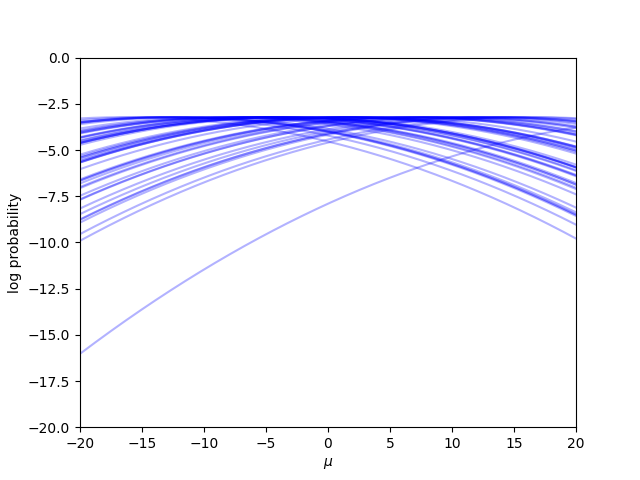
\includegraphics[width=\textwidth]{figs/background/logprob_var_10.png}
        \caption[]{$log(\vec{\theta}_a |\ \vec{y})$}
    \end{subfigure}
    \begin{subfigure}{0.475\textwidth}
        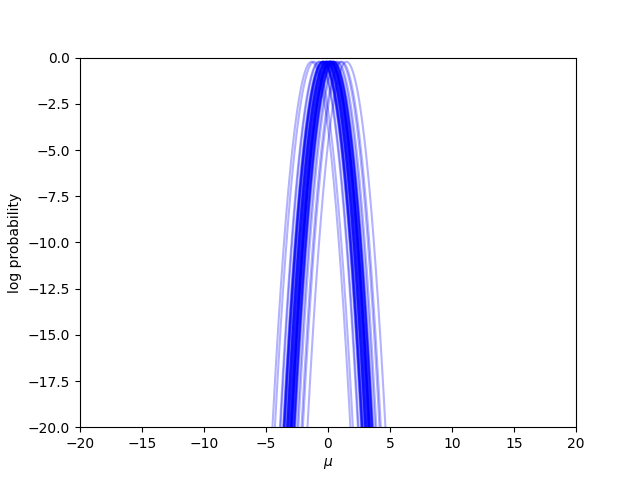
\includegraphics[width=\textwidth]{figs/background/logprob_var_0.5.png}
        \caption[]{$log(\vec{\theta}_b\ |\ \vec{y})$}
    \end{subfigure}
    \caption[Log-likelihood's of observations given a Gaussian distribution]{}
    \label{fig:loglikelihoods}
\end{figure}
\noindent Intuitively from these plots its clear that the low variance case a enables a more accurate estimation of $\mu$ due to the steeper slopes of the log-likelihood function. We obtain these slopes by taking derivative with respect to a model parameter ($\mu$ in this case) of the log-likelihood $\frac{\partial}{\partial\mu} log(\vec{\theta}\ |\ y),\;y\in\vec{y}$ this is known as the score function by convention, we will denote it as $\gls{score}$, note that for more complex functions we assume this derivative exists. For the sake of completeness we show plots of $\mathcal{S}_a$, $\mathcal{S}_b$ for our $\vec{y}$ observations from a and b respectively in \cref{fig:scorefunctions} and the distribution each score function $\mathbb{D}(\mathcal{S})$ when evaluated at the true parameter value $\mu' = 5$ in \cref{fig:scorefunctiondist}.
\begin{figure}
    \centering
    \begin{subfigure}{0.475\textwidth}
        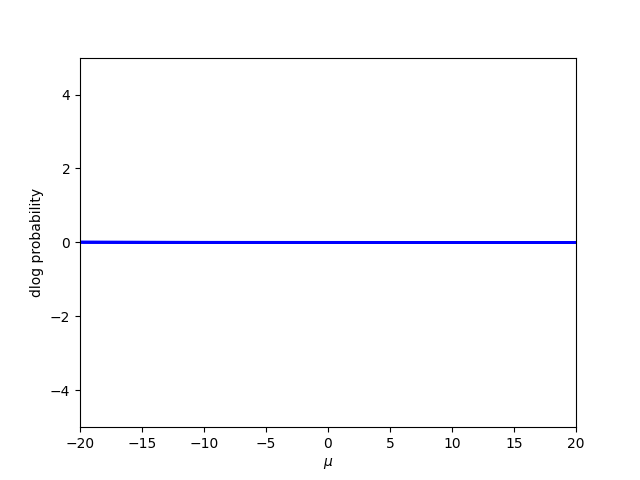
\includegraphics[width=\textwidth]{figs/background/deriv_var_10.png}
        \caption[]{$\frac{\partial}{\partial\mu} log(\vec{\theta}_a |\ \vec{y})$}
    \end{subfigure}
    \begin{subfigure}{0.475\textwidth}
        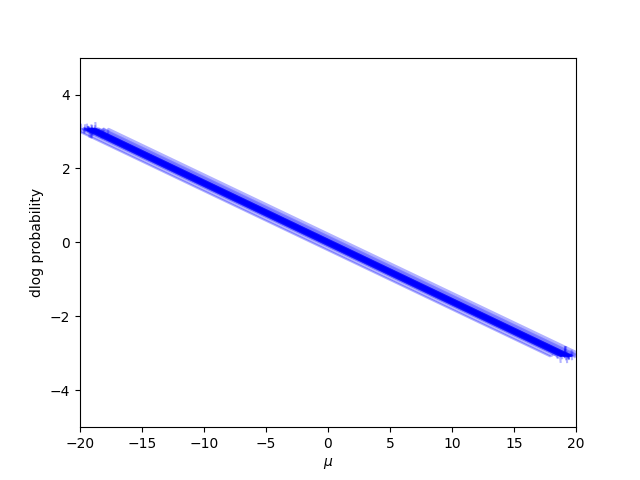
\includegraphics[width=\textwidth]{figs/background/deriv_var_0.5.png}
        \caption[]{$\frac{\partial}{\partial\mu} log(\vec{\theta}_a |\ \vec{y})$}
    \end{subfigure}
    \caption[Score functions of the log-likelihood of observations over $-20<x<20$]{}
    \label{fig:scorefunctions}
\end{figure}
\begin{figure}
    \centering
    \begin{subfigure}{0.475\textwidth}
        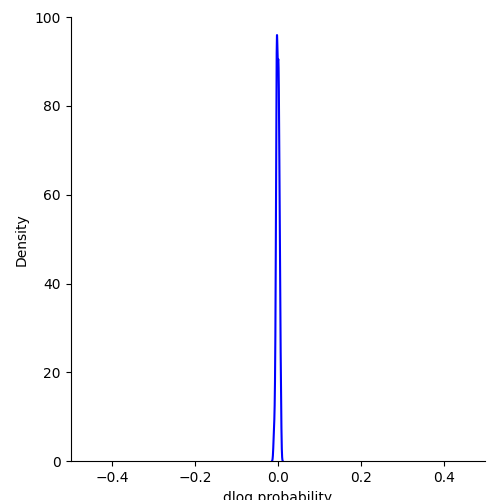
\includegraphics[width=\textwidth]{figs/background/deriv_dist_10.png}
        \caption[]{$\mathbb{D}\left(\frac{\partial}{\partial\mu} log(\vec{\theta}_a |\ \vec{y})\right), \mu'$}
    \end{subfigure}
    \begin{subfigure}{0.475\textwidth}
        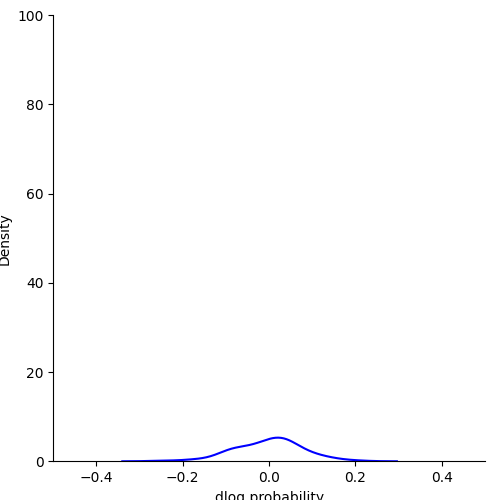
\includegraphics[width=\textwidth]{figs/background/deriv_dist_0.5.png}
        \caption[]{$\mathbb{D}\left(\frac{\partial}{\partial\mu} log(\vec{\theta}_a |\ \vec{y})\right), \mu'$}
    \end{subfigure}
    \caption[Distribution of the score functions when evaluated at $x=\mu'$ ]{}
    \label{fig:scorefunctiondist}
\end{figure}
\begin{equation}\label{eq:Fisherinfo}
    I(\theta) = -\EX_{\vec{\theta}} \left[
    \frac{\partial^2}{\partial^2\mu} log(y\ |\ \vec{\theta})\right]
\end{equation}
The Fisher information is given by the variance of the distribution of the score functions at the true parameter value $\VAR[\mathbb{D}(\mathcal{S}_a)], \mu'$. Calculating $I(\theta)$ from $\vec{y}$ we obtain $I(\theta_a)= 1.77\text{e}-5$ and $I(\theta_b)=5.37\text{e}-3$ confirming initial observations that the low variance case of b provides more information. Note as Fisher information is often used in cases where $\mu'$ is unknown, the secondary and more common method of calculation is to instead take the derivative of the score functions (second derivative of the log-likelihood), the fisher information in then given by \cref{eq:Fisherinfo}. As in a normal distribution the 2nd derivative of the log-likelihood is always a single value we omit plots of the second derivative and it's distribution when evaluated at $\mu'$ for brevity.
Now considering the multidimensional case of a complex system containing $X=\{x_1,x_2,\ldots,x_n\}$ random variables, each governed by a respective parameter in $\vec{\theta}=\{\theta_1,\theta_2,\ldots,\theta_n\}^T$. Let the value of a single element $x\in X$ in the system have the PDF $f(x\ |\ \theta_x) = y$, with a log-likelihood of $f_{x|\theta_x}(\vec{y}_x)$ where $\theta_x\in \vec{\theta}$ and $y_x$ is the set of observations we make of $x$. We make an additional assumption that that the score function $\forall x\in X,\; \gls{score}:=\frac{\partial}{\partial\mu} f_{x|\theta_x}(y_x)$ is finite (\ie $|X| = n < \infty$). The Fisher information matrix (FIM) \gls{fi} is then the row-major $n\times n$ matrix:
\begin{equation*}
    I(\vec{\theta}) = [I_{ij}(\vec{\theta})^{n}_{i,j=1}]
\end{equation*}
Where the jth element of the ith row is given by:
\begin{equation*}
    I_{ij}(\vec{\theta})= \EX_{\vec{\theta}} \left[
    \frac{\partial}{\partial \theta_i} log f_{x|\vec{\theta}}(y) \cdot
    \frac{\partial}{\partial \theta_j} log f_{x|\vec{\theta}}(y) \right]
\end{equation*}
\noindent This can be simplified by taking the second deviate in a similar fashion to \cref{eq:Fisherinfo} giving:
\begin{equation}\label{eq:FIM}
    I_{ij}(\vec{\theta})= -\EX_{\vec{\theta}}\left[
    \frac{\partial^2}{\partial \theta_i \partial \theta_j} log f_{x|\vec{\theta}}(y)\right]
\end{equation}
This matrix concisely represents the co-variance of all MLEs, with the co-variance of the $i$th and $j$th parameters estimator given by $\gls{fi}_{ij}$ and the variance of the estimator of parameter $n\equiv\gls{fi}_{nn}$.

\subsection{The Cramér–Rao Bound}
\label{ssec:Bcrb}

Given $I(\theta)$ the Cramér–Rao Bound (CRB) gives a lower bound on the accuracy with which we can estimate each $\theta\in\hat\theta$. From \cref{ssec:Bmle} we know that $\VAR(\gls{mle})$ dictates our confidence that the MLE reflects the true value of the parameter, it follows that the CRB is simply a bound on $\VAR(\gls{mle})$, we provide a proof from \cite{trees_detection_2013} under the assumption that the MLE is unbiased.
\begin{lemma}\label{lem:dx1}
Given an unbiased estimator $\int f\ dx=1$ 
\end{lemma}
\begin{align*}
    0 &= \EX[\hat\theta - \theta\ |\ \theta]\\
    &= \int (\hat\theta - \theta) f(x\ |\ \theta)dx\\
    &= \frac{\partial}{\partial\theta}\int \hat\theta - \theta) f(x\ |\ \theta)dx\\
    &= \int \hat\theta - \theta) f(x\ |\ \theta)\frac{\partial}{\partial\theta}dx-\int f\ dx\\
    &\therefore \int f\ dx = 1
\end{align*}
Using lemma 3.4.1 and the intuitive equality $\frac{\partial f}{\partial\theta} = f\frac{\partial log f}{\partial\theta}$ it follows:
\begin{equation}\label{eq:crbderivation}
\begin{aligned}
    \int(\hat\theta-\theta)\ \frac{\partial logf}{\partial\theta}dx = 1\\
    \int((\hat\theta-\theta)\sqrt{f})\cdot\left(\sqrt{f}\ \frac{\partial logf}{\partial\theta}\right) dx = 1\\
    \left[\int(\hat\theta -\theta)^2 f\ dx\right]\cdot
    \left[\int\left(\frac{\partial logf}{\partial\theta}\right)^2 f\ dx\right] \geq
    \left(\int((\hat\theta-\theta)\sqrt{f})\cdot
    \left(\sqrt{f}\ \frac{\partial logf}{\partial\theta}\right) dx\right)^2 = 1\\
\end{aligned}
\end{equation}
From rearranging the equality in \cref{eq:crbderivation} we have $\VAR(\hat\theta) \geq 1/I(\theta)$.\par
For the multi-parameter case of a FIM, instead of $\VAR(\widehat{\mathcal{L}})$, the CRB is w.r.t. the co-variance matrix $cov_\theta(\hat\theta)$ where $\hat\theta$ is the vector of MLE's for each  $\theta\in\vec{\theta}$ and $\vec{\theta}=\{\theta_1,\theta_2,\ldots,\theta_n\}^T$. The CRB is then given by the inequality $cov_\theta(\hat\theta)\geq \gls{fi}^{-1}$, we note that in cases where $n>>1$, $\gls{fi}^{-1}$ is infeasible to compute, in these cases a looser bound can be given using only the diagonal elements on the inverse matrix by $\sum_{i=1}^n 1/I(\hat\theta)_{ii}^{-1}$ as:
\begin{align*}
    \VAR_{\vec{\theta}}(\hat\theta) &= [cov_{\vec{\theta}}(\hat\theta)]_{ii}\\
    &\geq [I(\vec{\theta})]^{-1}_{ii}\\
    &\geq [I(\vec{\theta})_{ii}]^{-1}
\end{align*}

\section{Optimization Techniques}
\label{sec:Boptimization}
The accuracy of tomographic analysis is intuitively bound by the information acquired from measurements and how we process that information. In this section we introduce techniques for maximising the information we are able to gain from our probing. We decompose the measurement process into two stages: selection of paths to probe between monitor nodes and allocation of probes over these paths. In \cref{ssec:Bparsppselection} we address the first of these stages. We justify the desire for a minimal number of paths and present Zheng's algorithm for selecting this minimal set of paths. Next in \cref{ssec:Boptimumdesigns} we introduce concepts of optimum experimental design with the intent of using these to compute optimal probe allocation between paths in \cref{ssec:Mpallocation}.

\subsection{Parsimonious Probe Path Selection}
\label{ssec:Bparsppselection}

With a scope limited to tree network topologies \cite{lawrence_network_2006} focused on deriving an algorithm for an optimal selection of a set of probe paths $P^*$ for network tomography. We define an optimal selection of probe paths as the minimal set of probe paths that allow for complete node identifiability. Such a minimal set is desirable as when probing we allocate probe packets over each path $p\in P^*$, reducing the amount of information we gain about a path proportionally to the number of probe allocated to it. To ensure our inference is robust and has a maximal CRB (discussed in \cref{ssec:Bcrb}) we aim to gain as much data over the measurement interval as possible and adopt a parsimonious approach where we aim to select a $P^*$ s.t. \cref{eq:minpp} holds where $P$ is the set of all possible probe paths.
\begin{equation}
\label{eq:minpp}
    I(P^*) = I(P)
\end{equation}
\par
The problem of rigorously minimizing $P^*$ has been shown to be NP-hard by \cite{zheng_minimizing_2013}. However polynomial time solutions using a heuristic based approach for an approximation of a minimal $P*$ in general topologies have been derived previous and three notable methods have been developed: Zheng's algorithm (\cite{zheng_minimizing_2013}), Evolutionary Sampling algorithm (\cite{rahali_unicast_2019}), and Greedy-Min-Cost-Rank (\cite{tootaghaj_parsimonious_2018}). As the Evolutionary Sampling algorithm (ESA) was developed under the assumption of central monitors where all probe path metrics are compiled contrasting our assumption of observability of all monitors we do not consider ESA.\par
\captionsetup{justification=centering}
\begin{figure}[H]
    \centering
    \tikzsetnextfilename{bipartitegraph}
    \begin{tikzpicture}[
        node/.style={circle, draw=black!60, very thick, minimum size=5mm},
        group/.style={circle, draw=black!60, very thick, minimum size=5mm},]
        
        % Nodes
        \node[node] (v10) at (-6.5,1.5) {};
        \node[node] (v11) at (-5.5,1.5) {};
        \node at (-4.5,1.5) {{\LARGE\ldots}};
        \node[node] (v12) at (-3.5,1.5) {};
        
        \node[node] (u10) at (-6.5,-1.5) {};
        \node[node] (u11) at (-5.5,-1.5) {};
        \node at (-4.5,-1.5) {{\LARGE\ldots}};
        \node[node] (u12) at (-3.5,-1.5) {};
        
        \node[node] (v20) at (-0.5,1.5) {};
        \node[node] (v21) at (0.5,1.5) {};
        \node at (1.5,1.5) {{\LARGE\ldots}};
        \node[node] (v22) at (2.5,1.5) {};
        
        \node[node] (u20) at (-0.5,-1.5) {};
        \node[node] (u21) at (0.5,-1.5) {};
        \node at (1.5,-1.5) {{\LARGE\ldots}};
        \node[node] (u22) at (2.5,-1.5) {};
        
        % Groups
        \draw[dashed] (-5,1.6) ellipse (2.5cm and 0.75cm);
        \draw[dashed] (-5,-1.6) ellipse (2.5cm and 0.75cm);
        \draw[dashed] (1,1.6) ellipse (2.5cm and 0.75cm);
        \draw[dashed] (1,-1.6) ellipse (2.5cm and 0.75cm);
        
        % Edges
        \draw[very thick] (v10) -- (u10);
        \draw[very thick] (v10) -- (u11);
        \draw[very thick] (v11) -- (u12);
        \draw[very thick] (v11) -- (u10);
        \draw[very thick] (v12) -- (u12);
        \draw[very thick] (v20) -- (u11);
        \draw[very thick] (v20) -- (u12);
        \draw[very thick] (v21) -- (u22);
        \draw[very thick] (v20) -- (u20);
        \draw[very thick] (v22) -- (u21);
        \draw[very thick] (v22) -- (u22);
        
        % Labels
        \node at (-5,2) {$V_1$};
        \node at (-5,-2) {$U_1$};
        \node at (1,2) {$V_2$};
        \node at (1,-2) {$U_2$};
    \end{tikzpicture}
    \caption[Extended bipartite model of the network for probe path selection.]{Extended bipartite model of the network for probe path selection.}
    \label{fig:ebgm}
\end{figure}
Both Greedy-Min-Cost-Rank (GMCR) and Zheng's algorithm minimize the probing cost in a context analogous to ours, however the key difference is in definition of probing cost. In Zheng's algorithm the probing cost is defined as $|P^*|$ whereas in GMCR it is the total number of 'hops' or nodes in all paths $\forall p_i\in P^*,\ \sum |p_i|$. Although developed for the purpose of link tomography \cite{zheng_minimizing_2013} note it's applicability to node tomography we therefore adopt Zheng's algorithm \cref{alg:zhengs} for it's alignment with our goal of minimizing $|P^*|$. The core idea behind Zheng's algorithm is quantifying the contribution of a probe path to node identifiability and then adopting a greedy selection approach until all nodes are identifiable. The criteria used for the greedy is based on a novel extended bipartite graph model (EBGM) shown in \cref{fig:ebgm}.\par
This graph model groups network nodes into $V_1$ or $V_2$ based on if the node is identifiable or not. The group $U_1$ contains sets of probe paths that enable identification of a node in $V_1$, with an edge connecting a node in $V_1$ and $U_2$ if the set of paths in $U_2$ enables identification of $V_1$. Similarly $U_2$ contains probe paths which traverse a node in $V_2$, with an edge connecting a node in $V_2$ and $U_2$ if the path traverses that node.
\begin{algorithm}
    \KwData{The linear system $L$ and parameter $\alpha$}
    \KwResult{Minimal set of probe paths $P^*$}
    
    \For{each node}{
        Calculate $\alpha$ solutions using $A$ and $L$\;
    }
    Construct the extended bipartite graph $G'=(U,V,E)$ with the selected solutions\;
    $P^* \gets \varnothing$ \;
    $C \gets \varnothing$ \;
    \While{$\exists\ n \in V_1,\ n\not\in C$}{
        $u_{selected} \gets u_x\in U_1\ \text{with max}\left(\frac{|newV2|}{|newpaths|}\right)$ where: $newV2 = v_i\in V_2 - C,\ \{v_i, u_x\}\in E$ and $newpaths = p_i\in u_x,\ p_i \not\in P_s$\;
        $C \gets C + u_{selected}$\;
        $C \gets v_i \in V_1\cup V_2,\ \{v_i, u_{selected}\}\in E$\;
        \For {$p_i \in u_{selected}, p_i \not\in P^*$}{
            $P^* \gets P^* + p_i$\;
        }
    }
    \While{$\exists\ n \in V_2,\ n\not\in C$}{
        $u_{selected} \gets u_x\in U_1\cup U_2\ \text{with max}\left(\frac{|newV1|}{|newpaths|}\right)$ where: $newV1 = v_i\in V_1 - C,\ \{v_i, u_x\}\in E$ and $newpaths = p_i\in u_x,\ p_i \not\in P_s$\;
        $C \gets C + u_{selected}$\;
        $C \gets v_i \in V_1\cup V_2,\ \{v_i, u_{selected}\}\in E$\;
        \For {$p_i \in u_{selected}, p_i \not\in P^*$}{
            $P^* \gets P^* + p_i$\;
        }
    }
    Remove all replaceable probing paths from set $P^*$ using $L$\;
    \caption{Zheng's minimal probe path selection algorithm}
    \label{alg:zhengs}
\end{algorithm}

\subsection{Optimum Experiment Design}
\label{ssec:Boptimumdesigns}

Optimum experiment design (OED) is board field of study focusing on statistical methods to ensure an experiment yields the most robust and accurate results possible. Initially shepherded by \cite{smith_standard_1918}, of particular pertinence to tomography is OEDs applicability to parameter estimation in inverse problems. Work around OED for parameter estimation, as noted in \cref{cha:litreview}, primarily focuses on minimising the number of trials or "experimental cost" for accurately estimating a system's underlying statistical models, this lens can be inverted to instead maximise the accuracy of this estimation from a fixed number of trials.\par
At a high level, the problem of designing an optimal experiment is typically decomposed into 4 primary sub-problems: specification of a model, identification of the design region, specification of a design criterion, and specification of errors. If the formulated design differs significantly from popular existing approaches in literature a comparison should be drawn to validate key differences or identify missteps in problem specification. Irrelevant of its formulation, the experiment produces an estimator of the underlying parameters and is evaluated w.r.t the variance of this estimator as, intuitively, the variance of the estimator corresponds to the accuracy of the experiment.\par
Experiments to infer complex model\footnote{A complex model is analogous to the mathematical representation of a multi-parametric system such as a computer network.} parameters (sometimes referred to as screening experiments) can be evaluated using a range of statistical criteria however the two most common are A-optimality and D-optimality. A-optimality minimizes the average variance of all parameter estimates or, as the diagonal elements of the FIM correspond to these variances (\cref{ssec:Bfisherinformation}), the trace of the FIM tr$\left(\gls{fi}\right)$. In contrast D-optimality minimises the confidence region around the estimators, as this confidence region is inversely proportional to the determinant of the FIM (\cite{jones_-optimal_2021}) this is equivalent to maximising $|\gls{fi}|$.\par

\section{Summary}

In this chapter we have introduced four major concept areas critical to the understanding of network tomography. The ER and BA random graph generation algorithms were described in \cref{sec:Bgraphgeneration} and the key properties of the graphs they produce were highlighted. The scale-free nature of graph produced by the BA methods and the desirability of this property was covered. We additionally covered the relevance of techniques for generating large data sets to allow empirical validation in spite of the lack of availability of real world topologies.\par
In \cref{sec:Broutingmechanisms} we distinguish between general UDP network traffic (\textit{background traffic}) and \textit{probe packets} sent between monitored nodes. We describe four mechanisms which the routing of probe packets can be governed by and establish controllable cycle-free routing (\textit{CFR}) as the most applicable in the real world.\par
In \cref{sec:Bparameterestimation} we explain three related statistical concepts: maximum likelihood estimation, Fisher information, and the Cramér–Rao bound. We explain the use of each of these within inverse problems, specifically parameter estimation. In \cref{sec:Boptimization} we present concepts of parsimonious probe path selection and optimal experiment design. We then discuss the potential for both of these techniques to improve the accuracy of network tomography.
\chapter{Methodology}
\label{cha:methodology}
In this section we introduce our computational representation of networks along with concrete implementations and techniques used for dynamic routing algorithms and finally inference calculation...
\todo{Needs to be fleshed out once section complete}

\section{Optimizing Network Probing}
\label{sec:Moptprobing}
\subsection{Parsimonious Probe Path Selection}
\label{ssec:Mpppselection}

\subsection{Probe Allocation}
\label{ssec:Mpallocation}

As probes traversing different nodes and different probes traversing the same node have an independent effect on $q$ we can develop an aggregation of all measurements in $\vec{q}$ assuming $r\in R, q_r \sim \mathcal{N}(0, \theta_r)$ where the variance $\theta_r$ is unknown. Using this this we aim to infer an estimation of $\vec{\theta}$ from our monitor-to-monitor measurements $\vec{q}$. To formalise our knowledge of the network from probing we adapt a standard PDV PMF from \cite{he_network_2021} where $\mathcal{M} = \sum_{r\in p}\theta_r$ in \cref{eq:pdvobservationmodel} and denote the corresponding log-likelihood function as $\widehat{\mathcal{L}}(q, p)$.
\begin{equation}
\label{eq:pdvobservationmodel}
    f_{Q|\vec{\theta},\; \vec{\phi}}(q,\;p) = \phi_p \sqrt{2\pi\mathcal{M}}^{\ q^2/{2\mathcal{M}_r}}
\end{equation}
Using $\widehat{\mathcal{L}}(q, p)$ we are able to represent a network as a FIM, from this the CRB can be posed as a metric representing the lower bound on the accuracy of our inference, we elaborate on the specifics of this representation in \cref{sec:Mnetworkprobing}. Using this CRB however we can show that the equal allocation of probes over paths is a sub optimal approach to probing. Consider the example network in \cref{fig:fimex3routereg} we define three probe paths $p_0$, $p_1$, and $p_3$ traversing $r_0\rightarrow r_2$, $\ r_1\rightarrow r_2$, $\ r_0\rightarrow r_1\rightarrow r_2$, and the reserve directions respectively.
\begin{figure}[H]
    \centering
    \tikzsetnextfilename{3routertopology}
    \begin{tikzpicture}[
        router/.style={circle, draw=yellow!60, fill=yellow!5, very thick, minimum size=3.5mm},
        nef_router/.style={circle, draw=red!60, fill=red!5, very thick, minimum size=3.5mm},
        switch/.style={rectangle, draw=cyan!60, fill=cyan!5, very thick, minimum size=2.5mm},
        monitor/.style={rectangle, draw=magenta!60, fill=magenta!5, very thick, minimum size=2.5mm},]
        
        % Routers
        \node[router] (r0) at (-1.5,1.5) {$r_0$};
        \node[router] (r1) at (-1.5,-1.5)  {$r_1$};
        \node[router] (r2) at (1.5,0) {$r_2$};
        %Switches
        \node[monitor](s00) at (-3,1.5)   {$s_{0,0}$};
        \node[monitor](s10) at (-3,-1.5)   {$s_{1,0}$};
        \node[monitor](s20) at (3,0)   {$s_{2,0}$};

        %Links
        \draw[-] (r0.east) -- (r2.west);
        \draw[-] (r1.east) -- (r2.west);
        \draw[-] (r0.west) -- (s00.east);
        \draw[-] (r1.west) -- (s10.east);
        \draw[-] (r2.east) -- (s20.west);
        
        % Probe path visualizations.
        \node at (1,1.5) {$p_0$};
        \draw[dashed, line width=.5mm, <->] (-3,2.25) .. controls (0.5,2.5) and (0.5,0.25) .. (3, 0.5);
        \node at (1,-1.5) {$p_1$};
        \draw[dashed, line width=.5mm, <->] (-3,-2.25) .. controls (0.5,-2.5) and (0.5,-0.25) .. (3, -0.5);
        \node at (-0.75,0) {$p_3$};
        \draw[dashed, line width=.5mm, <->] (-3,0.75) .. controls (1.25,1.25) and (1.25,-1.25) .. (-3, -0.75);

    \end{tikzpicture}
    \caption{Example 3 router network with probe paths explicitly noted.}
    \label{fig:fimex3routereg}
\end{figure}

We examine three different probe allocations between [$p_0,\:p_1$]: $\phi_0$ = [0.33, 0.33, 0.33],  $\phi_1$ = [0.1, 0.8, 0.1], and $\phi_2$ = [0.8, 0.1, 0.1]. As there are no nefarious routers each router has an equal expected true PDV, let these true PDV's be $r_0=1, r_1=1, r_2=1$, the CRB of each probe allocation is then $\phi_0$=2.69, $\phi_1$=5.97, $\phi_2$=5.97. Recalling that the CRB provides a lower bound on inferential accuracy, the equal allocation of probes between paths results in the lowest inferential accuracy, this also holds when nefarious behaviour is included. Suppose the case of $r_1$ being nefarious with a $\frac{1}{3}$ probability of holding a packet any timestep, resulting in an increased PDV of 3 the CRB of each probing scheme is then $\phi_0$=1.51, $\phi_1$=4.24, $\phi_2$=2.05. Although each probing scheme performs worse it is clear that $\phi_0$ is comparatively even worse at detecting the increased PDV of the nefarious router than the case of no nefarious nodes. Note for comparison that in the previous case of being $r_1$ nefarious a pseudo optimal probing allocation $\phi_{optimal}$ = [0.0, 0.5, 0.5] results in a CRB of 33.67.

\section{Network Probing}
\label{sec:Mnetworkprobing}
    \begin{mdframed}\textbf{FROM BACKGROUND}\\
    In our context we can view these $\vec{\theta}$ as network properties or more productively - as a network is composed only of links and nodes - the link  and node level information which we are looking to infer from our analysis.
    Let a router's queuing delay \gls{qlen} have the probability distribution giving by the probability density function (PDF) $f_{Q|\theta_r}(q)$. We assume that that the derivative of the probability distribution $\partial f_{Q|\theta_r}(q)/\partial \theta_r$ exists and is finite (\ie $r = 1, ..., |R|$). The Fisher information matrix (FIM) is then the $|R|\times |R|$ matrix:

    \textbf{NOTATION FOR PDV SECTION FORMALIZATION}:
    Probe path probabilities: Each probe packet is sent along a probe path $p$ with a probability of $\phi_p$, given there are multiple paths within any non-trivial model we represent them all as $\vec{\phi}=\forall p\in P^*, \phi_p$ where $|\vec{\phi}|=|P^*|$, $\phi_p \geq 0$ and $\sum_{p\in P^*}\phi_p = 1$
    
    The parameter vector $\vec{\theta}$ is the vector of length $|R|$ containing the parameter governing each $q\in Q$ where $ q_x \sim \theta_x$ or more formally $\vec{\theta}=\forall r\in R, \theta_r$.
    
    The vector $\vec{\psi}$ is the vector containing all proper path allocations/injection probabilities where $\psi_x$ is the allocation of probes to $p_x\in P^*$ 
    
    Let $f_{Q|\vec{\theta}}(q)$ represent the probability of observing the value $q$ from monitor-to-monitor probe path $p\in P^*$ given the node parameter $\theta_x$ governing $Q_x$.
    
    Note that we can represent a tomographic problem as a system of $P^*f'(\theta)=\mathcal{M}$ where $f'$ is a one-to-one correspondence function of $\theta$ and $\mathcal{M}$ is a matrix of monitor-to-monitor metrics we collect from our probing where $\mathcal{M}_p = (q_1,q_2,\ldots, q_n)$. For ease of notation let $|\mathcal{M}_p|$ be the number of metrics ($n$) we collect over path $p$. Note that for aggregation of measurements after collection $\forall p\in P^*, \forall r\in p, \mathcal{M}=\sum_{r\in p}\theta_r$.
\end{mdframed}
    \todo{Integrate this into this section}

    To best utilise previous work on tomography we generalise our network as an $|\gls{routers}|\times|\gls{routers}|$ adjacent matrix where the $i$th$\times j$th entry is a 1 if those two routers are connected by a link and a 0 otherwise. Such an adjacency matrix is often referred to in network science as a routing matrix, as both terms are appropriate depending on circumstance we will use the terms interchangeable. Using this notation we are able to express the graph shown in \cref{fig:6routersample} where $M=\{s_{0,0},s_{5,0}\}$ as the adjacency matrix $A$:
    \begin{equation}\label{eq:6routeradjmatrix}
        A = \begin{bmatrix} 
            0 & 1 & 1 & 0 & 0 & 0 \\
            1 & 0 & 1 & 1 & 1 & 0 \\
            1 & 1 & 0 & 0 & 0 & 0 \\
            0 & 1 & 1 & 0 & 1 & 1 \\
            0 & 1 & 1 & 1 & 0 & 1 \\
            0 & 0 & 0 & 1 & 1 & 0 \\\end{bmatrix}
    \end{equation}
    
    \begin{figure}
        \centering
        \tikzsetnextfilename{6routertopology}
        \begin{tikzpicture}[
            router/.style={circle, draw=yellow!60, fill=yellow!5, very thick, minimum size=3.5mm},
            nef_router/.style={circle, draw=red!60, fill=red!5, very thick, minimum size=3.5mm},
            switch/.style={rectangle, draw=cyan!60, fill=cyan!5, very thick, minimum size=2.5mm},
            monitor/.style={rectangle, draw=magenta!60, fill=magenta!5, very thick, minimum size=2.5mm},]
            
            % Routers
            \node[router] (r0) at (-4.5,0)    {$r_0$};
            \node[router] (r1) at (-1.5,1.5)  {$r_1$};
            \node[router] (r2) at (-1.5,-1.5) {$r_2$};
            \node[router] (r3) at (1.5,1.5)   {$r_3$};
            \node[router] (r4) at (1.5,-1.5)  {$r_4$};
            \node[router] (r5) at (4.5,0)     {$r_5$};
            
            %Switches
            \node[monitor](s00) at (-6,.75)   {$s_{0,0}$};
            \node[switch] (s01) at (-6,-.75)  {$s_{0,1}$};
            \node[switch] (s10) at (-1.5,3)   {$s_{1,0}$};
            \node[switch] (s20) at (-1.5,-3)  {$s_{2,0}$};
            \node[switch] (s30) at (1.5,3)   {$s_{3,0}$};
            \node[switch] (s40) at (1.5,-3)   {$s_{4,0}$};
            \node[switch] (s50) at (6,.75)   {$s_{5,0}$};
            \node[monitor](s51) at (6,-.75)   {$s_{5,1}$};
            %Links
            \draw[-] (r0.east) -- (r1);
            \draw[-] (r0.east) -- (r2);
            \draw[-] (r1) -- (r2);
            \draw[-] (r1) -- (r3);
            \draw[-] (r1.south east) -- (r4.north west);
            \draw[-] (r2) -- (r3);
            \draw[-] (r2) -- (r4);
            \draw[-] (r3) -- (r4);
            \draw[-] (r3) -- (r5.west);
            \draw[-] (r4) -- (r5.west);
            \draw[-] (s00.east) -- (r0.west);
            \draw[-] (s01.east) -- (r0.west);
            \draw[-] (s10) -- (r1);
            \draw[-] (s20) -- (r2);
            \draw[-] (s30) -- (r3);
            \draw[-] (s40) -- (r4);
            \draw[-] (s50.west) -- (r5.east);
            \draw[-] (s51.west) -- (r5.east);
        \end{tikzpicture}
        \caption{6 router network with 2 monitors located at $r_0$ and $r_5$}
        \label{fig:6routersample}
    \end{figure}\par
    
    This method of network representation has several advantages for both practical implementation and theoretical analysis using tomographic methods. On the practicality front it interfaces seamlessly with prefab modules such as those provided by igraph and NS3 as well as our custom implementations of Dijkstra's algorithm. Consistent use of adjacency matrices for graph representation throughout all modules within the produced code base also allow for generalised use of the code for future analysis projects. On the analytical front this representation lends itself to computation of probe path matrices which are crucial for our method of gaining tomographic inference. \par
    As outlined in \cref{sec:Broutingmechanisms} we leverage assumed routing capabilities within existing network models to treat routing of probe packets from monitor nodes via probe paths uniquely from background traffic under CFR conditions. The set of probe paths used $\gls{p*}$ is represented using a $|\gls{p*}|\times |\gls{routers}|$ matrix where each row vector denotes routers within that probe path i.e. if the $j$th column of the $i$th row $= 1$ then router $j$ is present on probe path $i$ (0 otherwise). For the network represented in \cref{eq:6routeradjmatrix} we can denote a $\gls{p*}$ with a single probe path ($p_0$) traversing routers $r_0,r_1,r_4,r_5$ as:
    \[
        P'=\begin{bmatrix}
            1 & 1 & 0 & 0 & 1 & 1\\ 
        \end{bmatrix}
    \]
    Such a choice a $P$ would be useless however as it does not allow any router to be uniquely identified. To uniquely identify $r_1,r_2,r_3,r_4$ we require the probe path matrix with full column rank, such as:
    \begin{equation}
    \label{eq:6routerppaths}
        P^*=\begin{bmatrix}
                p_0 \\
                p_1 \\
                p_2 \\
                p_3 \\
                p_4 \\
        \end{bmatrix} = 
        \begin{bmatrix}
                1 & 1 & 0 & 0 & 1 & 1 \\
                1 & 1 & 0 & 1 & 0 & 1 \\
                1 & 1 & 0 & 1 & 1 & 1 \\
                1 & 0 & 1 & 0 & 1 & 1 \\
                1 & 1 & 1 & 0 & 1 & 1 \\
        \end{bmatrix}
    \end{equation}
    Using $P^*$ from \cref{eq:6routerppaths} we are able to compute a vector containing only $r_1$ through subtraction of row-vectors:
    \begin{align}
    \label{eq:r1computation}
        \begin{split}
            r_1 &= p_4-p_3\\
            &= \rowvect{1\;1\;1\;0\;1\;1} - \rowvect{1\;0\;1\;0\;1\;1}\\
            &= \rowvect{0\;1\;0\;0\;0\;0}\\
        \end{split}
    \end{align}\par
    As discussed in \cref{sec:Bpdvtomography} end-to-end metrics are collected over probe paths for the duration of the measurement interval. It follows from \cref{eq:r1computation} that we are able to use the observed values from our probing over paths 3 and 4 to infer properties of $r_1$. In the case of a fixed delay, in the vein of \cite{ma_efficient_2013}, we would calculate the difference in the mean of delay measurements from probe path 3 and probe path 4 to infer the delay of $r_1$. However as we aim to solve this problem for stochastic queuing delays the solution requires a more nuanced approach, we elaborate on our approach in \cref{sec:Mnefrouterdetection}.\par
    Note that given the network in \cref{eq:6routeradjmatrix} there exists no set $P' \subseteq \gls{ppaths}$ that allows for unique identification of $r_0$ or $r_5$ due to the CFR routing mechanism imposed. We refer to such routers within a graph that cannot be identified under the imposed routing mechanism onward as "unidentifiable". The set containing all unidentifiable routers within a network is denoted as \gls{urouters} and similarly the set of identifiable routers is denoted as \gls{irouters}, therefore the set of all routers $\gls{routers} = \gls{irouters}+\gls{urouters}$.\par
    Given this, we ignore \gls{urouters} and for $A$ in \cref{eq:6routeradjmatrix} we compute a vector containing each $r \in \gls{irouters}$ following conventions in \cref{eq:r1computation} to give the set of router level metrics \gls{metrics}:
    \begin{equation*}
        M = 
        \begin{cases}
        r_1, & p_4-p_3\\
        r_2, & p_4-p_0\\
        r_3, & p_2-p_0\\
        r_4, & p_2-p_1\\
        \end{cases}
    \end{equation*}
    Using this we are able to define router identifiability as:
    \begin{equation}
    \label{eq:identifiability}
        \forall r \in R_I,\;r \in M 
    \end{equation}
    Selection of an arbitrary $P^*$ where \cref{eq:identifiability} holds however is sub-optimal as we are required to split our probe packets between each $p\in P^*$. Intuitively we wish to gain as much data over the measurement interval as possible to ensure our inference is robust and as close to the CRB as possible (as discussed in \cref{ssec:Bfisherinformation}). We therefore adopt a parsimonious approach where we aim to select a $P^*$ s.t.
    \begin{equation}
    \label{eq:minpp}
        P^* = \argmin(f(P|A,CFR))
    \end{equation} 
    Where $P|A,CFR$ is an $|n|$x$|R|$ matrix of all possible ($n$) probe paths for a given routing matrix $A$ under CFR routing limitations and the function $f(P)$ computes the number of rows (probe paths) within $P$ required for full column rank for each non-unidentifiable router, resulting in uniquely identification of every possible router. We show how the use of this router level identification can be used to extend the example from \cref{ssec:Iex4router} to infer nefarious routers in \cref{sec:Mnefrouterdetection}.\par

\subsection{Parsimonious Probe Path Selection}
\label{ssec:Mparsppselection}
\todo{How we apply techniques from the content covered in background in our model.}
The choice of a minimal $P^*$ from \cref{eq:minpp} in a non-trivial task as established in \cref{ssec:Bparsppselection}. 

\section{Queue Stabilisation}
\label{sec:Mqueuestabilisation}
\todo{Describe how we generated results for steady queue lengths. Maybe remove this and just present in results as it's essentially just running the simulation and saving router level queue lengths each time step??}

\subsection{OSPF Routing}
\label{ssec:Mospfrouting}
\todo{Explain implementation of link state routing and update interval in the model.}

\section{Nefarious Router Detection}
\label{sec:Mnefrouterdetection}
\todo{Need to discuss how the addition of variables packet service time makes parameter estimation very inaccurate (even more so if transmission delays are employed)}

\section{Model Robustness}
\label{sec:Mmodelrobustness}
\todo{This subsection is to explain our method of varying the chance of a router delaying, the intensity of background traffic and topology to test the limits of our inferential accuracy.}

\section{Summary}
\todo{Once chapter is finished recap what we showed with a reference to each section.}

\chapter{Results and Discussion}
\label{cha:result}
In this section we apply techniques introduced in \cref{cha:methodology} to test our new methods for nefarious router classification. We present results of nefarious router classification under assumption sets one, two, and three in \cref{ssec:Ras1,ssec:Ras2,ssec:Ras3} respectively. We summarise our findings and comparisons between classifier in \cref{ssec:Rnefidsummary}. Comparisons focus on classifiers two and three as classifier one uses delay distribution not obtainable with network tomography. We then present results from testing of optimised probe path selection and probe allocation in \cref{sec:Rprobingoptimality}. Validation of model correctness with respect to assumptions regarding queue length stabilisation, noted as a requirement in previous work, is presented in Appendix A.

\section{Identifying Nefarious Behaviour}
\label{sec:Rnefarouterdetection}
For numerical analysis of classification under our proposed three assumption sets we consider the Nobel, Free, and CPLEX network topologies. This allows us to provide a robust analysis of analytical results using confusion matrices for each classification scenario. For each assumption set we discuss the classifiers performance under each scenario and provide generalised evaluations of each classifier, begin with assumption set one.

\subsection{Classifier One}
\label{ssec:Ras1}
Firstly we consider classification with a full delay distribution and baseline comparisons. Confusion matrices for nefarious node classification are shown in \cref{tab:ngercmatrix,tbl:frncecmatrix,tbl:nrwycmatrix}. Each classification was performed using a KS comparison against the true baseline values and a p-val cutoff of 0.0 to provide the strictly possible guarantee of significance.\par
\noindent
\begin{table}[H]
    \centering
    \aboverulesep = 0pt
    \belowrulesep = 0pt
    \begin{tabular}{l|cc}
        {\backslashbox{\textit{Actual}}{\textit{Predicted}}} & {Nefarious} & {Non-nefarious}\\
        \midrule
        {Nefarious}     & 1807  & 0     \\
        {Non-nefarious} & 37    & 3018  \\
    \end{tabular}
    \caption{Confusion matrix for classification under assumption set 1 in the Nobel topology.}
    \label{tab:ngercmatrix}
\end{table}
\noindent
\begin{table}[H]
    \centering
    \aboverulesep = 0pt
    \belowrulesep = 0pt
    \begin{tabular}{l|cc}
        {\backslashbox{\textit{Actual}}{\textit{Predicted}}} & {Nefarious} & {Non-nefarious}\\
        \midrule
        {Nefarious}     & 2781  & 101     \\
        {Non-nefarious} & 101    & 2658  \\
    \end{tabular}
    \caption{Confusion matrix for classification under assumption set 1 in the Free topology.}
    \label{tbl:frncecmatrix}
\end{table}
\noindent
\begin{table}[H]
    \centering
    \aboverulesep = 0pt
    \belowrulesep = 0pt
    \begin{tabular}{l|cc}
        {\backslashbox{\textit{Actual}}{\textit{Predicted}}} & {Nefarious} & {Non-nefarious}\\
        \midrule
        {Nefarious}     & 1905  & 46     \\
        {Non-nefarious} & 413   & 1896   \\
    \end{tabular}
    \caption{Confusion matrix for classification under assumption set 1 in the CPLEX topology.}
    \label{tbl:nrwycmatrix}
\end{table}
Classification in the Nobel topology has a sensitivity of 100\% across all evaluated sets of nefarious routers. With 37 false positives the classifier has a specificity of 99.99\%, giving an extremely precise and accurate nefarious node classification. For the Free and CPLEX topologies we observe marginally worse classification performance. The classifier has a sensitivity of 96.5\% and 97.64\% and a specificity of 96.34\% and 82.11\% for Free and CPLEX respectively. Given the efficacy of classification over all topologies we omit discussion under each scenario, as each would be near perfect, in favour of focusing on the general classification results and trends between topologies.\par
The most striking result is a sensitivity of 100\% in the Nobel topology, closely followed by the 99.9\% specificity in the same topology. We anticipate the extreme efficacy of this classification is due to the relatively small number of routers within the Nobel topology allowing us to obtain router identifiability using only 28 probe paths. The reduction in classifier performance as the size of the topology increases support this theory.\par
This trend is likely due to the number of probe paths required to achieve router identifiability in each topology. With fewer probe paths producing a robust average of metrics in each probe path. We would however expect the true sensitivity of the classifier to however be <100\% but the sample size needed to determine this would be prohibitively large.\par
In all topologies we observe the classifier having a higher sensitivity than specificity. This is likely due to the stochastic routing behaviour of the network routing packets away from nefarious routers which will have larger buffer queues. This would cause non-nefarious routers to receive more packets and subsequently a larger buffer queue appearing nefarious. Nefarious routers however - even when forwarded few packets - will still delay a proportion of these packet. These routers will therefore maintain a larger queue length, enabling their classification from packet delay metrics and minimising false negatives.\par

\subsection{Classifier Two}
\label{ssec:Ras2}
Next we consider classification with a baseline comparison and only packet delay summary statics available. ROC curves for classification in each topology are given in \cref{fig:RA2ROCcurves}. Note the performance of the classifier under each case is extrapolated from a corresponding point lying on the ROC curve.\par
For scenario one router classification in the Nobel, Free, and CPLEX topologies satisfied the sensitivity threshold of 0.9 with a false positive rate of 0.811, 0.838, and 0.919 respectively. Classification in the Nobel and Free topologies is superior to random classification of routers. However, with a sensitivity of > 0.763 the classification accuracy for the CPLEX network is worse than random. This is due to a sympathetic increase between non-nefarious router PDA (over baseline PDA) and nefarious router PDA. The sympathetic increase is caused by the link-state protocol routing packets around nefarious routers as their buffer queue's fill. This results in more packets being forwarded to non-nefarious routers over the baseline simulation, increasing the difference in PDA from the baseline simulation.\par
For scenario two the classifier reaches the 0.7 sensitivity threshold in the Nobel and Free within the specificity requirement but exceeds this requirement in the CPLEX topology with a false positive rate of 0.669. For scenario three the 0.9 specificity threshold is satisfied with a false negative rate of 0.558, 0.682, and 0.864 for each topology respectively.\par
In both scenario two and three all classifier perform better than a random classification. However for scenario two classification in the CPLEX topology is notably worse than the Nobel and Free topologies, even when accounting for the increased number of routers. We anticipate this is caused by the same factors as in scenario one, likely increased noise in probe path measurements. In general however less stringent sensitivity requirements reduce the impact of noise on classification.\par
With scenario three's requirements on specificity the reduction in classifier accuracy is proportional to the number of routers in each topology. Additionally across all topologies the classifier performs the best relative to a random classification in sensitivity and specificity ranges of [0.2, 0.76] and [0.24, 0.83] respectively. Classification under assumption case two is therefore better suited to use cases with a higher tolerance for false negatives.\par
\noindent
\begin{figure}[H]
    \centering
    \begin{subfigure}{0.475\textwidth}
        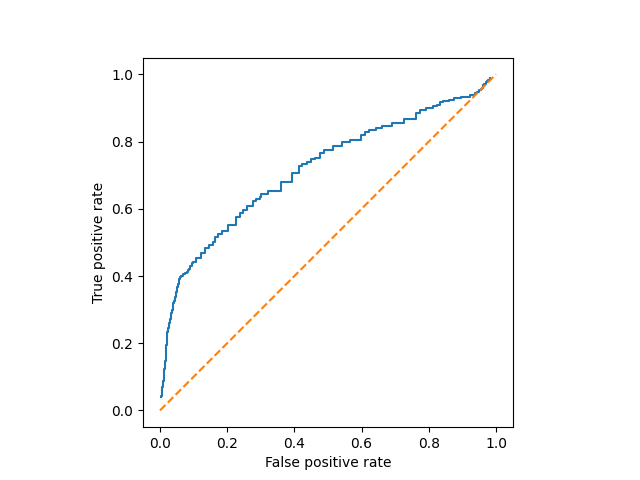
\includegraphics[width=\textwidth]{figs/results/nobel-germany_case2_roc.png}
        \caption{Nobel Topology.}
    \end{subfigure}
    \begin{subfigure}{0.475\textwidth}
        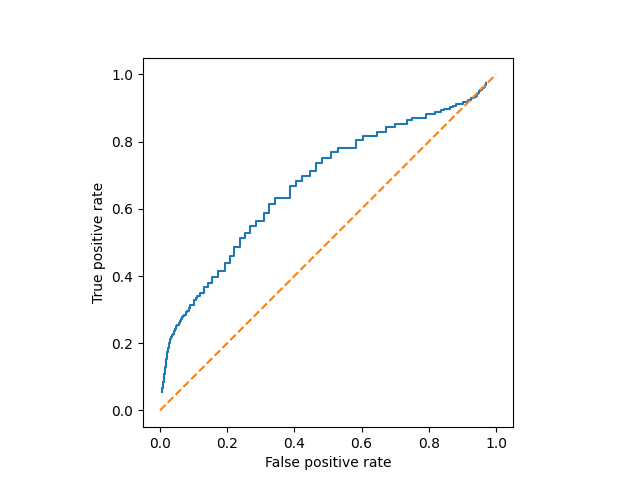
\includegraphics[width=\textwidth]{figs/results/france_case2_roc.png}
        \caption{Free Topology.}
    \end{subfigure}
    \begin{subfigure}{0.475\textwidth}
        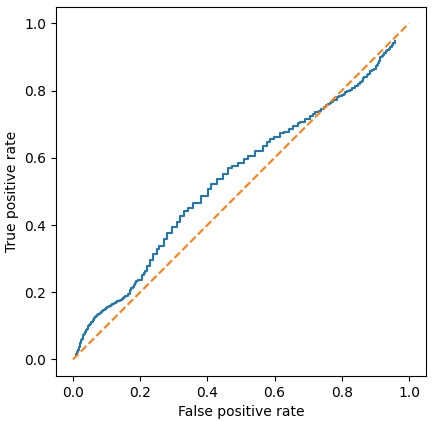
\includegraphics[width=\textwidth]{figs/results/norway_case2_roc.png}
        \caption{CPLEX Topology.}
    \end{subfigure}
    \caption{ROC curves for classification under assumption set 2.}
    \label{fig:RA2ROCcurves}
\end{figure}

\subsection{Classifier Three}
\label{ssec:Ras3}
\noindent
\begin{figure}
    \centering
    \begin{subfigure}{0.475\textwidth}
        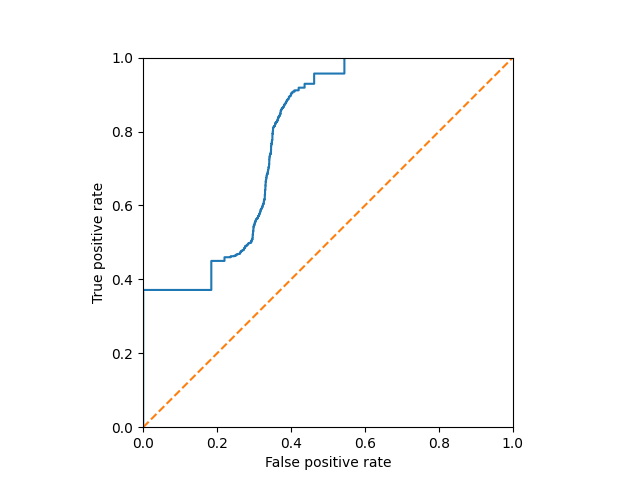
\includegraphics[width=\textwidth]{figs/results/nobel-germany_case3_roc.png}
        \caption{Nobel Topology.}
    \end{subfigure}
    \begin{subfigure}{0.475\textwidth}
        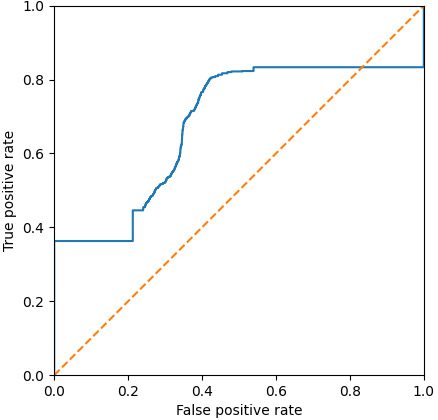
\includegraphics[width=\textwidth]{figs/results/france_case3_roc.png}
        \caption{Free Topology.}
    \end{subfigure}
    \begin{subfigure}{0.475\textwidth}
        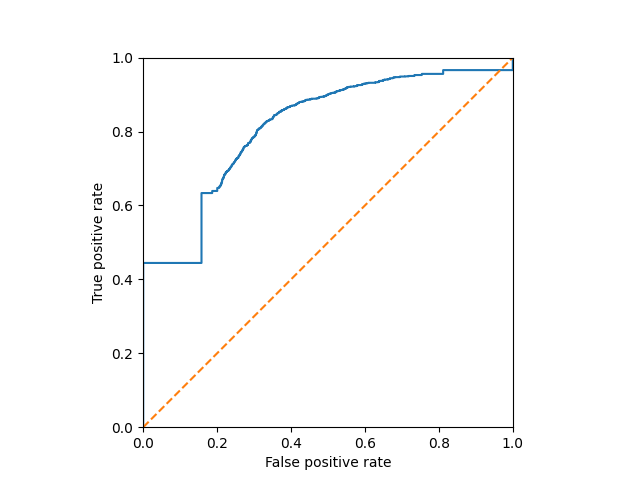
\includegraphics[width=\textwidth]{figs/results/norway_case3_roc.png}
        \caption{CPLEX Topology.}
    \end{subfigure}
    \caption{ROC curves for classification under assumption set 3.}
    \label{fig:RA3ROCcurves}
\end{figure}
Finally we use only packet delay summary statics for classification. ROC curves for classification in each topology are given in \cref{fig:RA3ROCcurves}. We evaluate the classifiers performance for each scenario below.\par
For scenario one classification of the Nobel and CPLEX topologies results in a false positive rate of 0.4 and 0.5 respectively. For the Free topology the classifier is only able to attain a sensitivity of 0.9 with a false negative rate of 1.0 (classify all routers as nefarious). Excluding this case, PDA is not sufficient to classify routers with a sensitivity greater than 0.83 in the Free topology.\par
This is due to the topology containing a node with a degree of 10 (Paris). The Paris node experiences more than twice as much traffic as the average node of degree 3 and thus has a near or completely full queue buffer regardless of nefarious behaviour. This is compounded by 15 of the 37 probe paths including Paris, resulting in a disproportionate number of probe packets traversing the router. Therefore when using a PDA threshold of buffer queue length $-\epsilon$ for classification the Paris node is always classified as nefarious. A similar limitation exists in the CPLEX topology where due to the same factors where a maximum sensitivity of 0.966 can be achieved.\par
Conversely, the classifier performs extremely well on the Nobel topology achieving a true positive rate of 1.0 with a false positive rate of 0.544. Although both Nobel and CPLEX have a maximum node degree of 6, in the Nobel network only 12 probe paths traverse the maximally connected router compared to 21 in CPLEX. Therefore in the CPLEX network, unlike the Free network, the maximally connected router's buffer queue receives disproportionately more probe packets. This results in the router being classified as nefarious regardless of its delaying behaviour in the majority of test trials.\par
For scenario two classification of all topologies meets specificity requirements with classification in the Nobel, Free, and CPLEX topologies having a false positive rate of 0.339, 0.363, and 0.235 respectively. These rates are a strict improvement over those from classifier two. This improvement is due to the increased queue length of nefarious routers causing traffic to be re-routed through non-nefarious routers, increasing their queue lengths. As this sympathetic increase is absent in the baseline simulation, an increase in PDA is seen from non-nefarious router's baseline. This increase is indistinguishable from the buffer queue increase in nefarious routers. Therefore, there we observe more cases of routers being incorrectly labeled as nefarious.\par
For scenario three classification of each topology results in a false negative rate of 0.629 for the Nobel and Free topologies and 0.556 for CPLEX. However, for each case in \cref{fig:RA3ROCcurves} no PDA thresholds enable a classification with a false positive rate < 0.2. This is due to an overlap in PDA values between weakly connected nefarious router and strongly connected non-nefarious routers. The amount of traffic arriving at strongly connected non-nefarious routers fills their buffer queue at a rate similar to a less connected nefarious router. Therefore, any PDA threshold sufficient to identify any weakly connected nefarious routers incorrectly labels strongly connected non-nefarious routers.\par

\subsection{Summary of Comparisons}
\label{ssec:Rnefidsummary}
In this section we have analysed three nefarious routers classifiers with three real-world use cases for a fair comparison of performance. Classifier one was found to have the best performance in each use case. This classifier achieved a near perfect accuracy across all investigated topologies. However, as this underlying distribution can not be obtained via network tomography we focused our comparison on the second and third classifiers.\par
Classifier two was found to perform better than a random classification in all cases other than in the CPLEX topology with a sensitivity > 0.763. This was caused by a sympathetic increase between non-nefarious router PDA (over baseline PDA) and nefarious router PDA due to stochastic traffic routing. This classifier performed optimally for specificity requirements between 0.24 and 0.83 across all topologies.\par
Classifier three achieved greater accuracy than classifier two for sensitivity and specificity requirements of [0.2, 0.83] and [0.46, 0.75] respectively. This was due to absence of baseline comparisons causing sympathetic increases between routers to not impact classification. However, classifier two performed very poorly for sensitivities below 0.2 and above 0.8. This was due to an overlap in PDA metrics between strongly connected non-nefarious and weakly connected nefarious.

\section{Optimisation Impacts}
\label{sec:Rprobingoptimality}
In this section we apply optimization techniques for selection of probe paths between monitor nodes and allocation of probe packets between paths. Inference made under optimized conditions are compared and contrasted to original measures to quantify impact of optimizations, computational costs involved in optimization techniques are weighed against changes in accuracy to assess the practicality of implement these improvements in tomographic monitoring schemes.

\subsection{Proportional Probe Allocation}
\label{ssec:Rprobeallocation}
In \cref{fig:RprobeoptROCcurves} we present results from classification with PDA inferred from network tomography. Sub-figures a, c, and e correspond to classifier two and sub-figures b, d, and f correspond to classifier three. Classifier one is not included in our analysis here as the information it requires cannot be obtained via network tomography. In each sub-figure a ROC curve showing classification accuracy is provided for both unoptimised and optimised proportional probe allocation (PPA) over paths.\par
An equivalent or improved classification accuracy is achieved using PPA for both classifiers over all topologies compared to unoptimised probing. This is most apparent in sub-figures a, b, and e where PPA results in a mean sensitivity improvement of 0.214, 0.204, and 0.1 respectively over all false positive rates.\par
This means that for any set maximal tolerance of false positive we are on average able to correctly classify 17\% more nefarious routers using network tomography with PPA. Improvements can also be seen in sub-figure f where PPA enables classification with a minimum false positive rate of 5\% compared to only 50\% without optimisation.\par
This improvement in classifier performance with PPA for the Nobel and CPLEX topologies is due to the variation of routers between probe paths. For both the Nobel and CPLEX topologies a single router is present in at most 25\% of paths however in the Free topology a single router is present in at most 47\% of probe paths. This means that with a proportion allocation this singular router in the Free topology receives disproportionately more packets. Many of these additional probe packets are dropped due to the limited queue buffer, resulting in only minor changes in classification accuracy from the PPA.\par
\noindent
\begin{figure}[H]
    \centering
    \begin{subfigure}[H]{0.475\textwidth}
        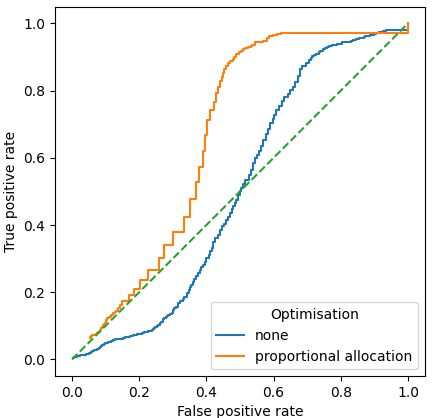
\includegraphics[width=\textwidth]{figs/results/nobel-germany_ac2_opt.png}
        \caption{Nobel Topology Classifier 2.}
    \end{subfigure}
    \begin{subfigure}[H]{0.475\textwidth}
        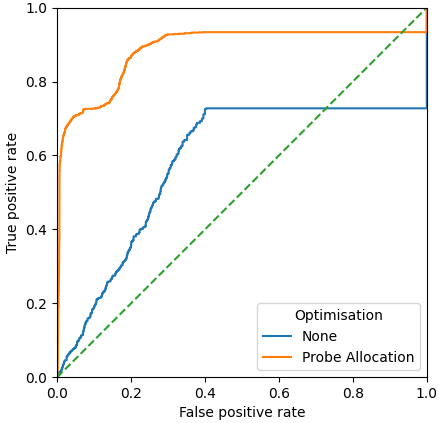
\includegraphics[width=\textwidth]{figs/results/nobel-germany_ac3_opt.png}
        \caption{Nobel Topology Classifier 3.}
    \end{subfigure}
    \begin{subfigure}[H]{0.475\textwidth}
        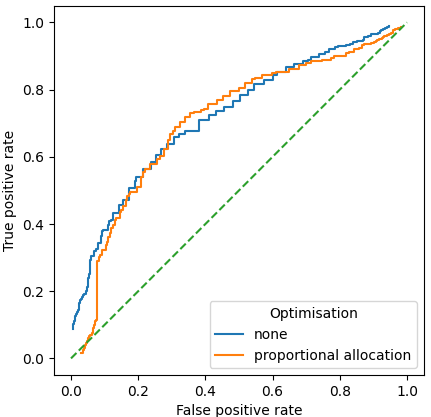
\includegraphics[width=\textwidth]{figs/results/france_ac2_opt.png}
        \caption{Free Topology Classifier 2.}
    \end{subfigure}
    \begin{subfigure}[H]{0.475\textwidth}
        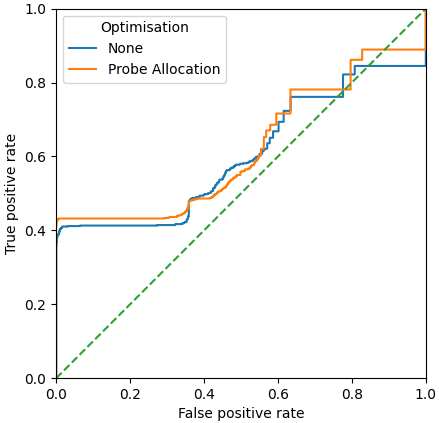
\includegraphics[width=\textwidth]{figs/results/france_ac3_opt.png}
        \caption{Free Topology Classifier 3.}
    \end{subfigure}
    \begin{subfigure}[H]{0.475\textwidth}
        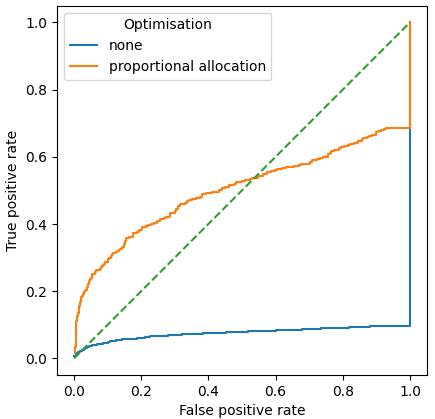
\includegraphics[width=\textwidth]{figs/results/norway_ac2_opt.png}
        \caption{CPLEX Topology Classifier 2.}
    \end{subfigure}
    \begin{subfigure}[H]{0.475\textwidth}
        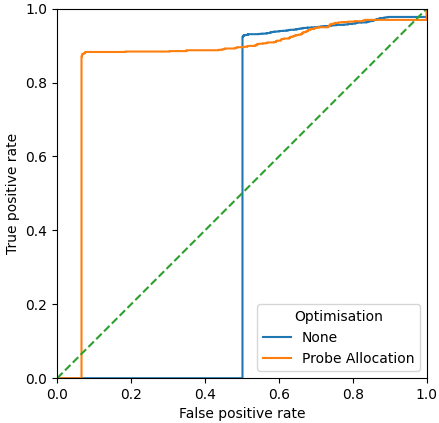
\includegraphics[width=\textwidth]{figs/results/norway_ac3_opt.png}
        \caption{CPLEX Topology Classifier 3.}
    \end{subfigure}
    \caption{ROC curves for optimised classification.}
    \label{fig:RprobeoptROCcurves}
\end{figure}
In sub-figure a, for false positive rates < 0.5 classification with unoptimised probe allocation is worse than random. This result is unlikely to be due to noise as it has been average over many simulation runs. We speculate that this poor classification is potentially due to the buffers of nefarious routers being comprised of solely probe packets. This could potentially be caused by traffic re-routing around these nefarious routers. PDA measurements would therefore be far lower than would be expected if background traffic was also being forwarded to these routers. However, additional investigation into this behaviour in future work is required to form a substantiated explanation.

\subsection{Lower Accuracy Bound}
\label{ssec:Rloweraccuracybounds}
Results from analytical calculation of the CBR given probe paths and probe allocation for each topology are given in \cref{tbl:crbs}. In each case the CRB is extremely low, this is due to the large number of probe paths used in tomography for each topology. However, as this only represent a lower bound we focus on comparison of the CRB between topologies and each probe allocation scheme in a topology.\par
For both probe allocations network tomography in the Nobel topology has the highest CRB. Probing the in the Free and CPLEX topologies was calculated to have the second highest and lowest CRB respectively. This corresponds to classifier accuracy evaluation from ROC curves of each classifier in \cref{fig:RprobeoptROCcurves}. This decrease in accuracy is proportional to the increase in number of routers in each each topology. This is due to the additional probe paths required to uniquely identify each router reducing the number of measurements we are able to take over each path.\par
However, under PPA probing the larger CPLEX network has a higher CRB than the Free network. This is due to the Free topology containing a router with a degree of ten which a disproportionate number of probe paths traverse. Under PPA more probe packets are sent to this router, causing more to be dropped as its buffer queue is already at capacity. These dropped probe packets are the cause of this decrease in the lower accuracy bound.\par
Comparing probing scheme within topologies, the CRB of network tomography with PPA is greater than with an unoptimised probe allocation for each topology. The improvement in accuracy of network tomography in the Nobel and CPLEX topologies is 2.07e-4 and 7.92e-6, however, for the Free topology the improvement is only -4.9e-7.\par
\begin{table}[H]
 \centering
  \begin{tabular}{@{}ccc@{}}
   \toprule
    &\multicolumn{2}{c}{\textbf{Probe Allocation}}\\
    \cmidrule(rl){2-3}
    Topology & Unoptimised & PPA \\
    \midrule
    Nobel & 3.18e-05 & 2.39e-04\\
    Free & 1.42e-06 & 1.91e-06\\
    CPLEX & 1.94e-07 & 8.11e-06\\
   \bottomrule
  \end{tabular}
  \caption{Calculated Cramér–Rao bound for each topology and probe allocation}
  \label{tbl:crbs}
\end{table}
This is consistent with ROC curves in \cref{fig:RprobeoptROCcurves} where a significant improvement in classification was observed for the Nobel and CPLEX topologies. Additionally, the smaller difference in CRB between probe allocation schemes for the Free topology corresponds with classifier performance, where the smallest difference between probe allocation schemes was observed.\par


\subsection{Metric Normalisation}
\label{ssec:Rmetricnormilisation}
ROC curves for nefarious router classification with PDA normalised w.r.t. router degree are shown in \cref{fig:RmetricnormROCcurves}. We omit classifier one as it does not use PDA for classification. For classifier two, a decrease in accuracy across all true and false positives rates is seen. Similarly, for classifier three an equal or lesser accuracy over all topologies is seen.\par
The general decrease in classification accuracy is likely due to a router's degree being a poor representation of the number of packets it receives each timestep. Other contributing factors such as the routing tables of surrounding routers and their respective degree would also likely need to be accounted for. It is also possible that the contributions of incoming traffic and nefarious delaying to a routers queue length are intrinsically related.\par
This means that attempts to account for incoming traffic contributions to better identify nefarious delaying are unlikely to yield classification improvements irrelevant of the number of factors relating to incoming traffic volume are accounted for. We therefore highlight methods of distinguishing between incoming traffic, and other factors which contribute to a router's buffer queue size, to better identify nefarious delaying behaviour as an area for future research.\par
\noindent
\begin{figure}[H]
    \centering
    \begin{subfigure}[H]{0.475\textwidth}
        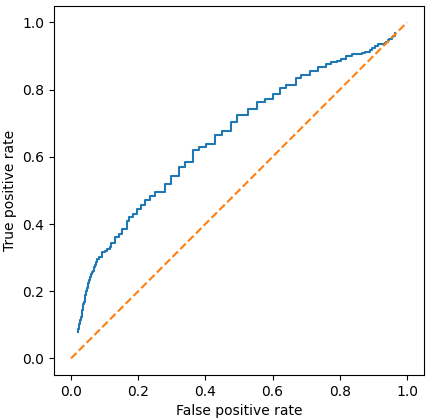
\includegraphics[width=\textwidth]{figs/results/metric_normilisation/nobel-germany_ac2.png}
        \caption{Nobel Topology Classifier 2.}
    \end{subfigure}
    \begin{subfigure}[H]{0.475\textwidth}
        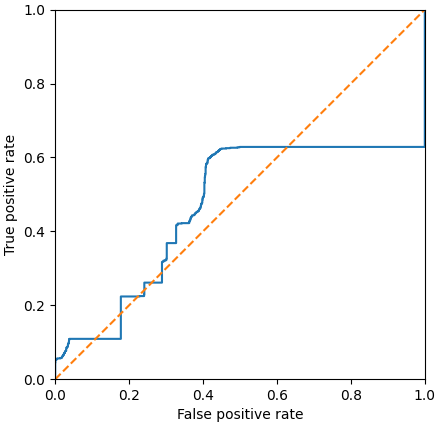
\includegraphics[width=\textwidth]{figs/results/metric_normilisation/nobel-germany_ac3.png}
        \caption{Nobel Topology Classifier 3.}
    \end{subfigure}
    \begin{subfigure}[H]{0.475\textwidth}
        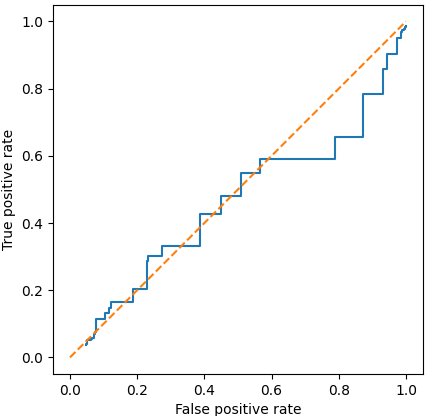
\includegraphics[width=\textwidth]{figs/results/metric_normilisation/france_ac2.png}
        \caption{Free Topology Classifier 2.}
    \end{subfigure}
    \begin{subfigure}[H]{0.475\textwidth}
        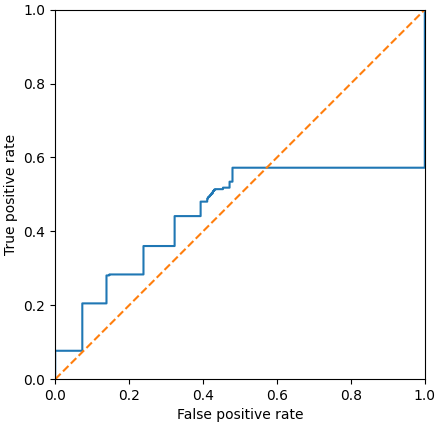
\includegraphics[width=\textwidth]{figs/results/metric_normilisation/france_ac3.png}
        \caption{Free Topology Classifier 3.}
    \end{subfigure}
    \begin{subfigure}[H]{0.475\textwidth}
        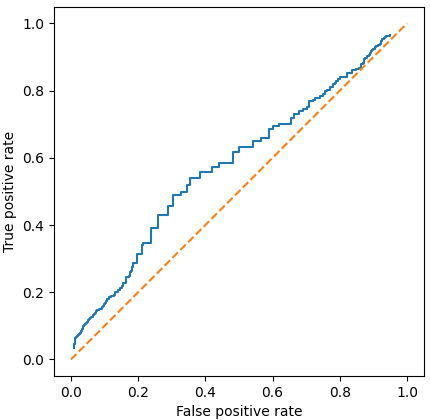
\includegraphics[width=\textwidth]{figs/results/metric_normilisation/norway_ac2.png}
        \caption{CPLEX Topology Classifier 2.}
    \end{subfigure}
    \begin{subfigure}[H]{0.475\textwidth}
        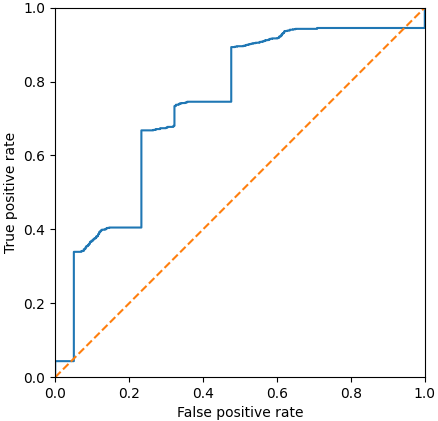
\includegraphics[width=\textwidth]{figs/results/metric_normilisation/norway_ac3.png}
        \caption{CPLEX Topology Classifier 3.}
    \end{subfigure}
    \caption{ROC curves for optimised classification.}
    \label{fig:RmetricnormROCcurves}
\end{figure}

\section{Summary}

\chapter{Conclusion}
\label{cha:conc}
Research into the use of network tomography in real-work networks is limited, with most studies being conducted on synthetic topologies. Additionally, in previous work that has focused on applying network tomography to real-world scenarios, there is little investigation into adversarial settings. In this thesis we have addressed this gap in the corpus, through studying the classification of nefariously delaying routers in stochastically routing real-world networks. This probabilistic delaying of packets by routers could be indicative of a compromised router snooping data using DPI or ex-filtrating packets.\par
We have proposed the technique of \textit{PDA tomography}, a novel implementation of network tomography, to infer the size of a router's packet queue buffers in a stochastically routing network. This implementation computes the average packet delay over a set of controllable cycle-free probing paths through the network. We have established a relationship between average packet delays and packet delaying behaviour.\par
We have developed two classifiers which use PDA tomography to identify nefarious routers in a network. One classifier was developed under the assumptions that log files exist allowing for comparison of observed router PDAs to a PDA of the routers when not exhibiting nefarious delaying behaviour. The other classifier does not assume these log files are available, and uses router PDA alone to identify nefarious routers.\par
The classifier using a comparison to baseline metrics was found to be effective in identifying nefarious routers with a false positive rate < 0.2 and a false negative rate of < 0.2. The classifier which uses PDA alone was found to have a more accurate classification of nefarious routers outside of these sensitivity and specificity ranges.\par
To optimise the accuracy of our classification of nefarious routers, we introduced two candidate optimisations to the tomographic pipeline. The first of these, proportional probe allocation (PPA), was found to improve the accuracy of both classifiers across all topologies. Observations of classifier performance under PPA were found to corroborate analytical results from calculation of the Cramér–Rao bound. The lower bound on accuracy of network tomography, given by the Cramér–Rao bound, was improved by PPA in each topology. Additionally, the Cramér–Rao bound decreased proportional to the number of routers in topology, for both equivalent probe allocation and PPA.\par
The second optimisation was intended to account for the impact of inbound traffic on a router's queue buffer length. This would allow for the more accurate identification of changes in router queue buffer size due to nefarious delaying. To accomplish this the PDA of each router was normalised by the degree of the router. This was found to negatively impact the performance of both classifiers across all topologies. We hypothesise that this negative impact on classifier performance is due to the degree of a router being insufficient to account for the impact of incoming traffic on a routers buffer queue length.\par

\section{Future Work}
\label{sec:Cfuture}
While this thesis has provided a foundation for the use of network tomography to classify nefarious routers, there are many areas for potential future improvements. Studies conducted around the impact of alternative background routing protocols and advanced attacks, such as OSPF poisoning, would greatly expand the scope of this work. A very promising area for future work would be investigation into the use of a combination of PDA and PDV metrics in advanced classification techniques, such as K-nearest neighbours. Additionally, an approach utilising PDV alone would, additionally, resolve complications surrounding clock synchronisation between monitors in real-world applications.\par
Further research into the impact of alternative probe allocation optimisation algorithms such as Greedy-Min-Cost-Rank (GMCR) and the Evolutionary Sampling algorithm (ESA) could further improve classification accuracy. Specifically, use of ESA would allow for a distributed approach to PDA tomography, accounting for the collation time of metrics when allocating probes between paths.\par
Additional research building on our work focusing on mapping router level PDA to hold probability (in Appendix B) has much potential. Specifically, analysis into if the underlying parametric functions which relate these two metrics is robust enough to be inverted. The sensitivity of this relationship to network topology, traffic intensity, and alternate network properties could also hold promise.\par 
An analysis using a network simulation software package, such as NS3, could be used to investigate the impact of a TCP rather than UDP based network. If real-world network traffic data sets with probabilistically delaying routers could be obtained, future analysis of this method's efficacy in real-world settings could be studied. Larger real-world topologies could also be analysed to see if our observations of classifier efficacy hold for networks where many more probe paths are required.\par
Discretisation of packet delay metrics obtained from network tomography into segments throughout the measurement interval could be attempted in future work. This could generate a distribution closer to the underlying router buffer queue length distribution. As seen in results for classifier one, buffer queue length distribution classification is extremely precise and accurate when using the underlying true router buffer queue length. Shifting the results of the tomographic analysis towards this PDA distribution could potentially improve accuracy.\par
Additional work evaluating of our hypothesis, as to why normalisation of router PDA by router degree does not improve inferential accuracy, is also warranted. Such research into alternative methods of distinguishing the contributing factors to router PDA could, additionally, result in a more accurate classification of nefarious routers.


%%%%%%%%%%%%%%%%%%%%%%%%%%%%%%%%%%%%%%%%%%%%%%%%%%%%%%%%%%%%%%%%%%%%%%
% Here begins the end matter

\appendixpage
\appendix
\chapter*{Appendices}
\addcontentsline{toc}{chapter}{List of Appendices}
\renewcommand{\thesection}{\Alph{section})}
\renewcommand{\thesubsection}{\Alph{section}.\arabic{subsection}}

\section{Verbose Queue Length Stabilisation Results Over LS Update Intervals}
\subsection{Average Queue Length}
    \begin{figure}[h]
        \centering
        \begin{subfigure}[b]{0.475\textwidth}
            \centering
            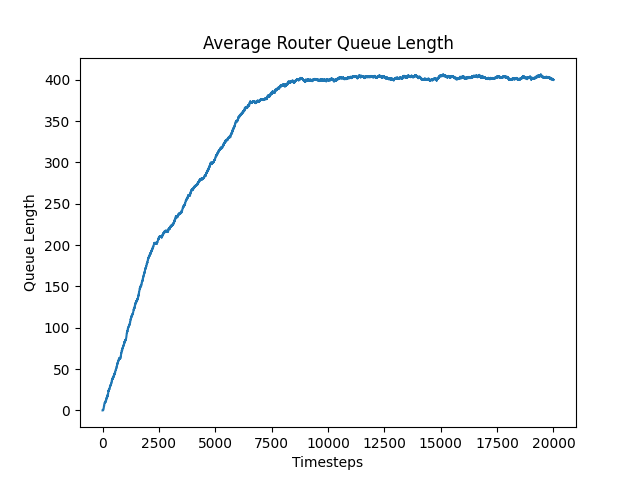
\includegraphics[width=\textwidth]{figs/appendix/average_ls=1.png}
            \caption[]{Average router queue length (LS update interval = 1)}
        \end{subfigure}
        \hfill
        \begin{subfigure}[b]{0.475\textwidth}
            \centering
            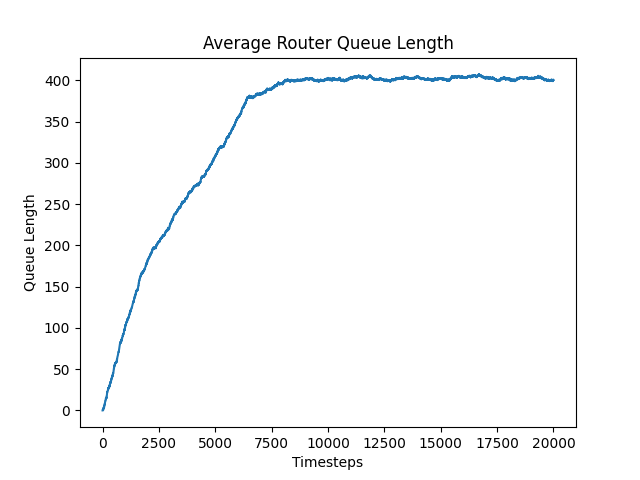
\includegraphics[width=\textwidth]{figs/appendix/average_ls=10.png}
            \caption[]{Average router queue length (LS update interval = 10)}
        \end{subfigure}
    \end{figure}
    \begin{figure}[H]\ContinuedFloat
        \centering
        \begin{subfigure}[b]{0.475\textwidth}
            \centering
            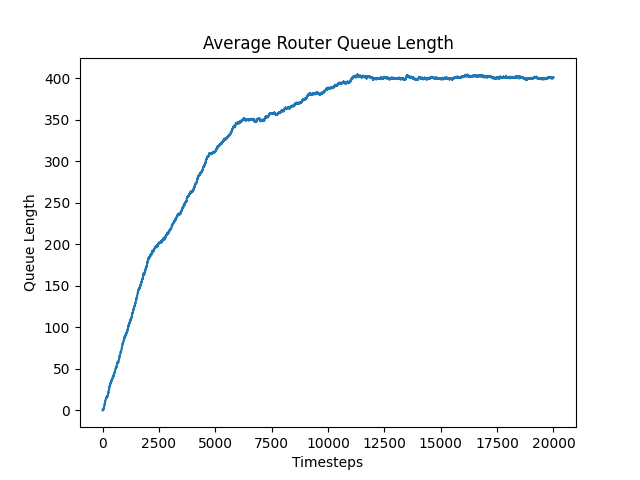
\includegraphics[width=\textwidth]{figs/appendix/average_ls=50.png}
            \caption[]{Average router queue length (LS update interval = 250)}
        \end{subfigure}
        \hfill
        \begin{subfigure}[b]{0.475\textwidth}
            \centering
            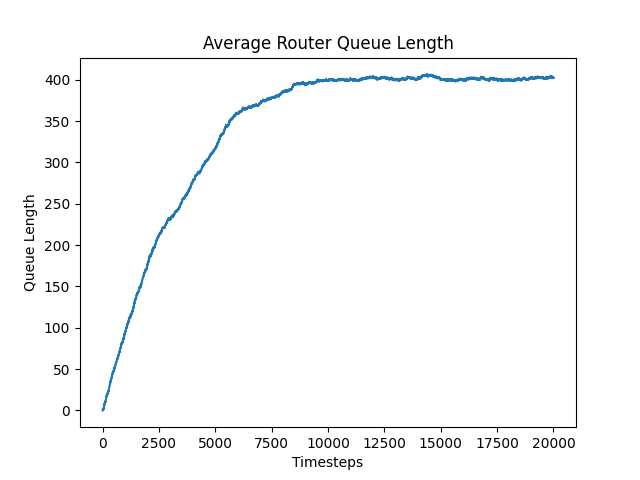
\includegraphics[width=\textwidth]{figs/appendix/average_ls=500.png}
            \caption[]{Average router queue length (LS update interval = 500)}
        \end{subfigure}
    \end{figure}
    \begin{figure}[H]\ContinuedFloat
        \centering
        \begin{subfigure}[t]{0.475\textwidth}
            \centering
            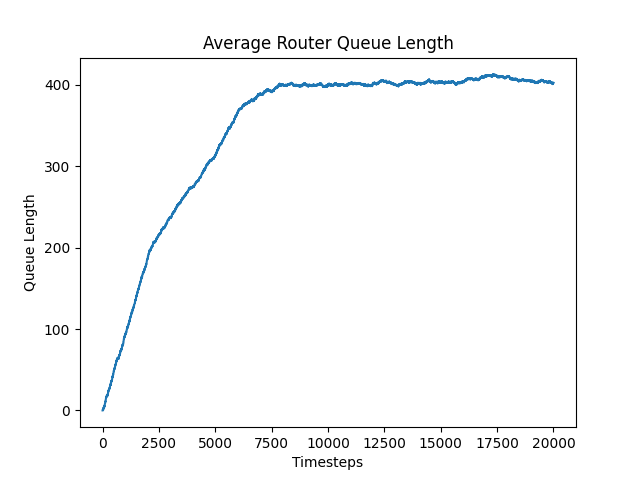
\includegraphics[width=\textwidth]{figs/appendix/average_ls=1000.png}
            \caption[]{Average router queue length (LS update interval = 1000)}
            \label{fig:avgq-1000}
        \end{subfigure}
        \hfill
        \begin{subfigure}[t]{0.475\textwidth}
            \centering
            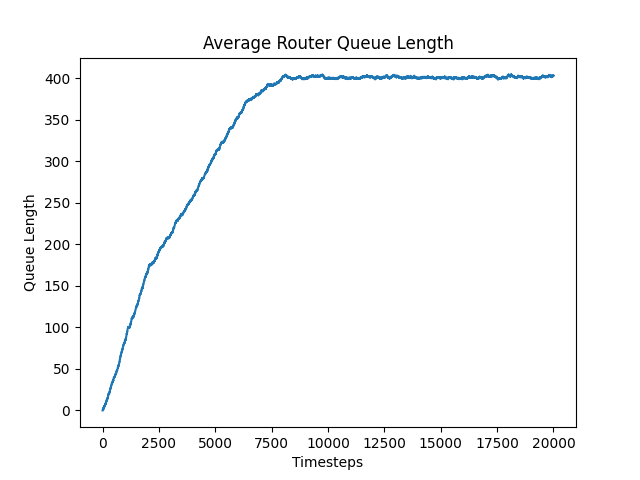
\includegraphics[width=\textwidth]{figs/appendix/average_ls=10000.png}
            \caption[]{Average router queue length (LS update interval = 10000)}
            \label{fig:avgq-10000}
        \end{subfigure}
    \end{figure}
    
\subsection{Variance of Queue Length}
\lfix{Trim variance graphs to same length as averages}
    \begin{figure}[H]
        \centering
        \begin{subfigure}[b]{0.475\textwidth}
            \centering
            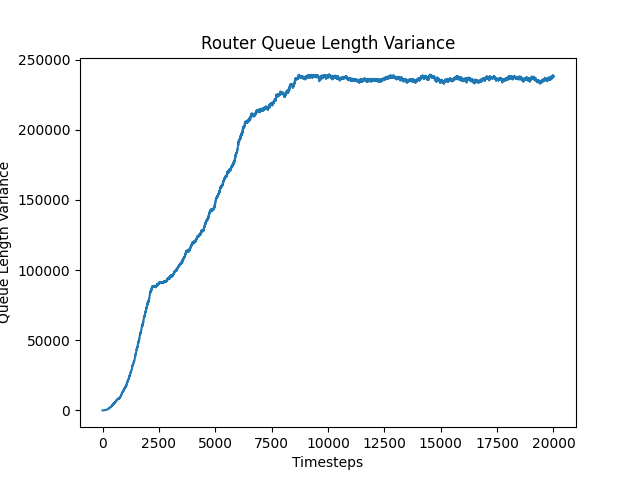
\includegraphics[width=\textwidth]{figs/appendix/variance_ls=1.png}
            \caption[]{Variance of router queue length (LS update interval = 1)}
            \label{fig:qvar-1}
        \end{subfigure}
        \hfill
        \begin{subfigure}[b]{0.475\textwidth}
            \centering
            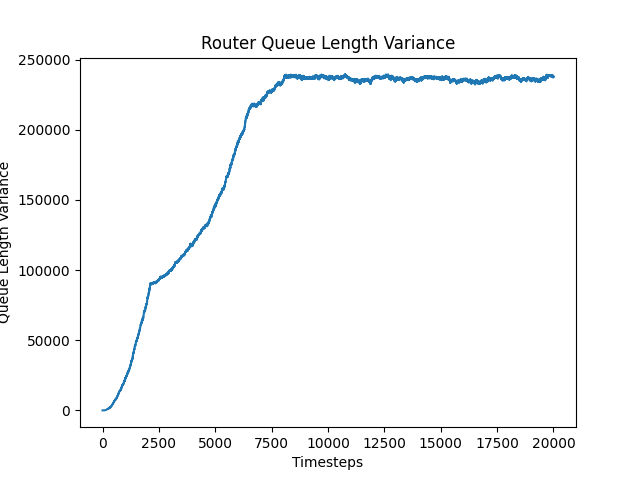
\includegraphics[width=\textwidth]{figs/appendix/variance_ls=10.png}
            \caption[]{Variance of router queue length (LS update interval = 10)}
            \label{fig:qvar-10}
        \end{subfigure}
    \end{figure}
    \begin{figure}[H]\ContinuedFloat
        \centering
        \begin{subfigure}[b]{0.475\textwidth}
            \centering
            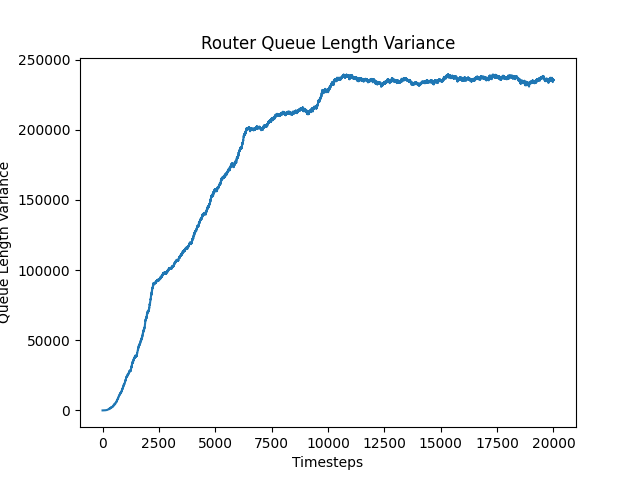
\includegraphics[width=\textwidth]{figs/appendix/variance_ls=250.png}
            \caption[]{Variance of router queue length (LS update interval = 250)}
            \label{fig:qvar-250}
        \end{subfigure}
        \hfill
        \begin{subfigure}[b]{0.475\textwidth}
            \centering
            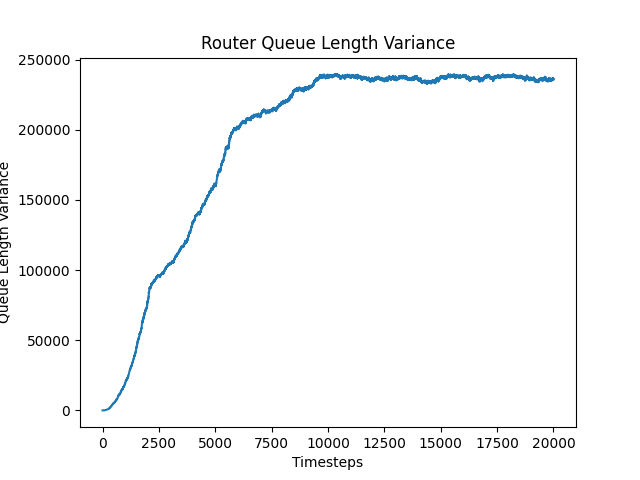
\includegraphics[width=\textwidth]{figs/appendix/variance_ls=500.png}
            \caption[]{Variance of router queue length (LS update interval = 500)}
            \label{fig:qvar-500}
        \end{subfigure}
    \end{figure}
    \begin{figure}[H]\ContinuedFloat
        \begin{subfigure}{0.475\textwidth}
            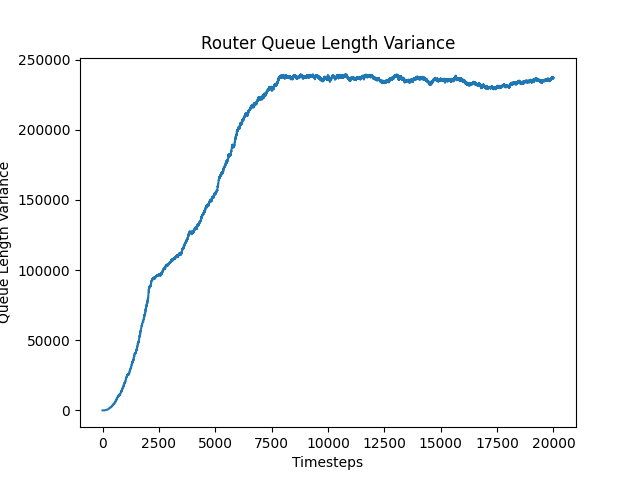
\includegraphics[width=\textwidth]{figs/appendix/variance_ls=1000.png}
            \caption[]{Variance of router queue length (LS update interval = 1000)}
            \label{fig:qvar-1000}
        \end{subfigure}
        \hfill
        \begin{subfigure}[H]{0.475\textwidth}
            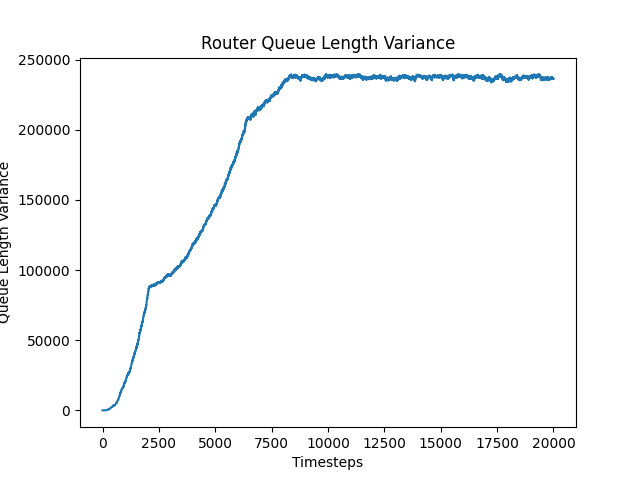
\includegraphics[width=\textwidth]{figs/appendix/variance_ls=10000.png}
            \caption[]{Variance of router queue length (LS update interval = 10000)}
            \label{fig:qvar-10000}
        \end{subfigure}
    \end{figure}

\newpage

\newpage
\section{Queue Stabilization}
\label{sec:Aqueuestabilization}

\todo{Describe how we generated results for steady queue lengths, implementation of link state routing and update interval in the model}

\captionsetup{justification=centering}
\begin{figure}[H]
    \centering
    \begin{subfigure}{0.475\textwidth}
        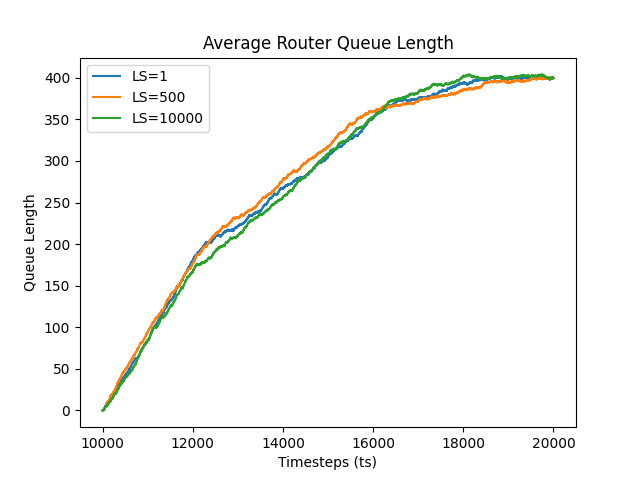
\includegraphics[width=\textwidth]{figs/results/average_of_1,500,10000.png}
        \caption{Average router queue buffer length.}
        \label{fig:Ravgq}
    \end{subfigure}
    \hfill
    \begin{subfigure}{0.475\textwidth}
        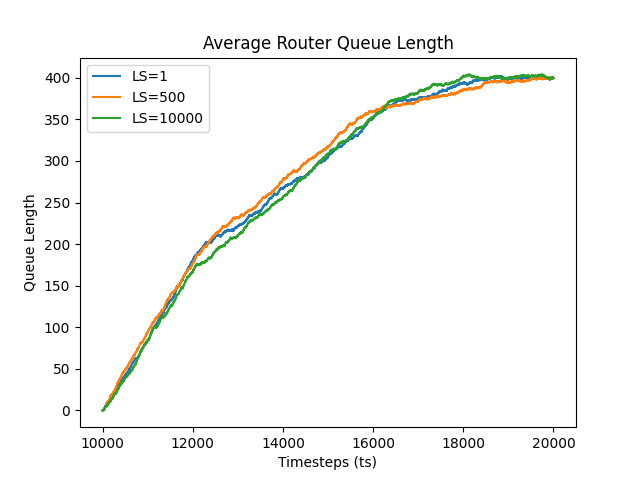
\includegraphics[width=\textwidth]{figs/results/average_of_1,500,10000.png}
        \caption[]{Variance of router queue buffer length.}
        \label{fig:Rvarq}
    \end{subfigure}
    \caption{Mean and variance of router queue buffer lengths over link-state update intervals 1, 500, and 10,000].}
\end{figure}

\begin{table}[H]
    \centering\sisetup{table-number-alignment=center}
    \begin{tabular}{@{}lS[table-format=1.2e1]c@{}}
        \toprule
        \multirow{2}{*}{\makecell{LS Update \\ Interval}} & \multicolumn{2}{@{}S@{}}{\textbf{Time-step range}}\\
        \cmidrule(rl){2-3}
        & {$\leq$ 20,000} & {> 20,000} \\
        \midrule
        1       & 1.07E4 & 6.25 \\ 
        10      & 1.02e4 & 4.88 \\
        50      & 1.01e4 & 3.21 \\
        250     & 1.07e4 & 5.06 \\
        500     & 1.01e4 & 6.05 \\
        1,000   & 1.03e4 & 3.47 \\
        10,000  & 1.12e4 & 5.22 \\
        \bottomrule
    \end{tabular}
    \caption{Variance pre and post queue length stabilization point}
\end{table}

\newpage

\newpage
\section{Sympathetic Packet Delay Metric Increase}
\label{sec:Asympathicpdv}
Note symmetric increase due to topology symmetry.

\newpage
\section{Curve Fitting with Alternative Minimisation Algorithms}
\label{Aaltcurvefit}
\begin{figure}[H]
    \centering
    \begin{subfigure}{0.475\textwidth}
        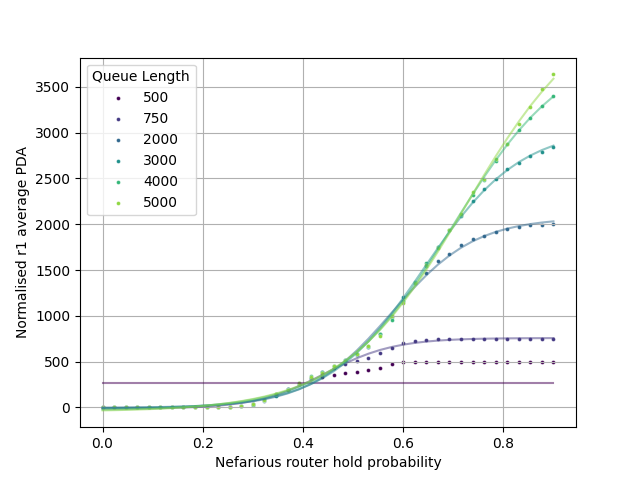
\includegraphics[width=\textwidth]{figs/results/qlen_fitting/qlen_PDA_trf.png}
        \caption{Original}
    \end{subfigure}
    \begin{subfigure}{0.475\textwidth}
        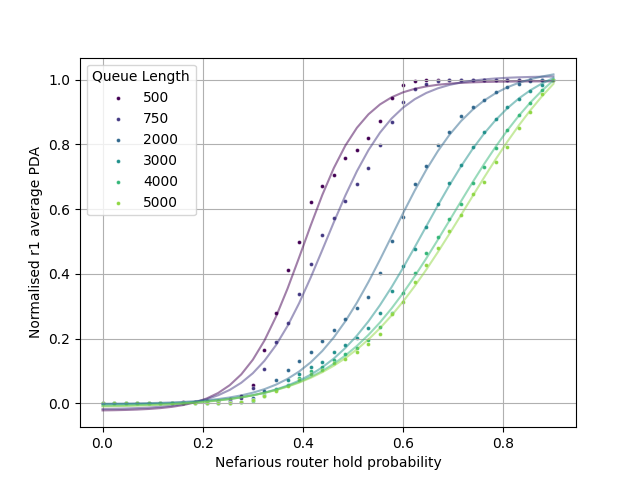
\includegraphics[width=\textwidth]{figs/results/qlen_fitting/norm_qlen_PDA_trf.png}
        \caption{Min-max scaled}
    \end{subfigure}
    \caption{Plots of average nefarious router buffer queue length over various hold probabilities fitted using TRF minimisation.}
\end{figure}

\begin{figure}[H]
    \centering
    \begin{subfigure}{0.475\textwidth}
        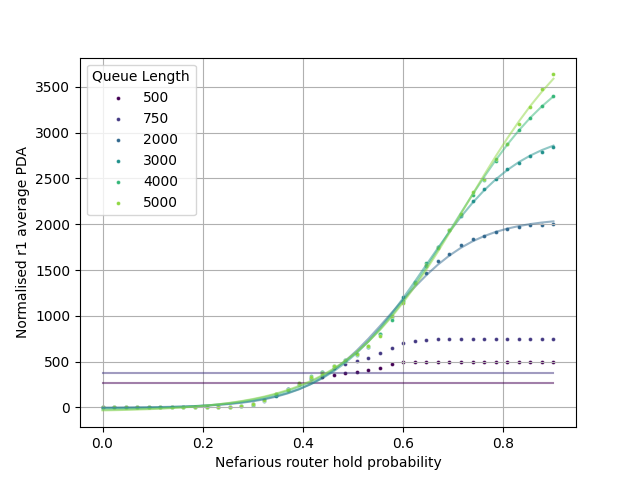
\includegraphics[width=\textwidth]{figs/results/qlen_fitting/qlen_PDA_dogbox.png}
        \caption{Original}
    \end{subfigure}
    \begin{subfigure}{0.475\textwidth}
        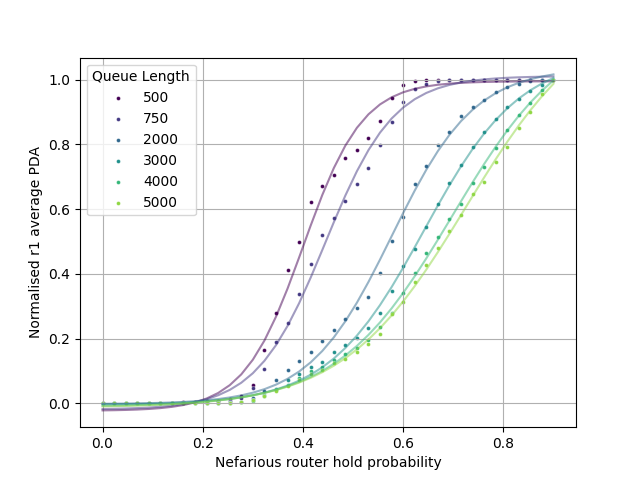
\includegraphics[width=\textwidth]{figs/results/qlen_fitting/norm_qlen_PDA_dogbox.png}
        \caption{Min-max scaled}
    \end{subfigure}
    \caption{Plots of average nefarious router buffer queue length over various hold probabilities fitted using dogbox minimisation.}
\end{figure}

\begin{table}[H]
 \centering
  \begin{tabular}{@{}cccccc@{}}
   \toprule
    &&\multicolumn{2}{c}{\textbf{PDA}} & \multicolumn{2}{c}{\textbf{PDV}} \\
    \cmidrule(rl){3-4} \cmidrule(rl){5-6}
    Algorithm & $R^2$ & Original & Scaled & Original & Scaled \\
    \midrule
    \multirow{2}{*}{LM}     & $\overline{x}$ & 99.778        & 99.778 & 99.187 & 99.187 \\
                            & min            & 99.403        & 99.403 & 98.323 & 98.323 \\
    \multirow{2}{*}{TRF}    & $\overline{x}$ & 83.211        & 99.778 & -      & 99.187 \\
                            & min            & 5.679         & 99.403 & -      & 98.323 \\
    \multirow{2}{*}{Dogbox} & $\overline{x}$ & 66.595        & 99.778 & -      & 99.187 \\
                            & min            & 6.399$e^{-9}$ & 99.403 & -      & 98.323 \\
   \bottomrule
  \end{tabular}
  \caption{Variance of nefarious router PDA grouped by varying delay probabilities in the baseline 6 router network. (Note all values are $R^2\cdot 100$)}
\end{table}

\backmatter

\bibliographystyle{anuthesis}
% \nocite{*}
\bibliography{thesis}

\printindex

\end{document}
